% =============================================================================
% intercalar.tex — Relatório Intercalar · ForensiQ · UC 21184
% Universidade Aberta · Licenciatura em Engenharia Informática · 2025/26
% Orientador: Prof. Pedro Duarte Pestana
% Autor: João Rodrigues (2203474)
% Compilar: latexmk -pdf -cd src_latex/intercalar.tex
% =============================================================================

\documentclass[a4paper,11pt]{article}

% --- Codificação e tipografia -----------------------------------------------
\usepackage[utf8]{inputenc}
\usepackage[T1]{fontenc}
\usepackage{lmodern}
\usepackage{microtype}
\usepackage{textcomp}

% --- Layout -----------------------------------------------------------------
\usepackage[top=2.5cm,bottom=2.5cm,left=3cm,right=2.5cm]{geometry}
\usepackage{parskip}
\usepackage{setspace}
\onehalfspacing

% --- Matemática --------------------------------------------------------------
\usepackage{amsmath}
\usepackage{amssymb}

% --- Tabelas, listas, arrays ------------------------------------------------
\usepackage{booktabs}
\usepackage{longtable}
\usepackage{array}
\usepackage{multirow}
\usepackage{enumitem}
\setlist{nosep,leftmargin=1.5em}

\newcolumntype{L}[1]{>{\raggedright\arraybackslash}p{#1}}

% --- Imagens, cores, caixas -------------------------------------------------
\usepackage{graphicx}
\usepackage{rotating}  % sidewaysfigure para diagramas verticais grandes
\graphicspath{{figures/}{../docs/architecture/diagrams/}}

\usepackage[dvipsnames,svgnames,table]{xcolor}
\definecolor{primaryblue}{RGB}{21,101,192}
\definecolor{successgreen}{RGB}{46,125,50}
\definecolor{warningorange}{RGB}{230,81,0}
\definecolor{dangerred}{RGB}{198,40,40}

\usepackage{tcolorbox}
\tcbuselibrary{skins,breakable}
\newtcolorbox{infobox}[1]{
    colback=blue!5,colframe=primaryblue!60,
    fonttitle=\bfseries\small,title=#1,
    breakable,
}

% --- Código-fonte (listings) ------------------------------------------------
\usepackage{listings}
\lstset{
    basicstyle=\ttfamily\footnotesize,
    breaklines=true,
    frame=single,
    backgroundcolor=\color{gray!8},
    rulecolor=\color{gray!40},
    captionpos=b,
    numbers=left,
    numberstyle=\tiny\color{gray},
    keywordstyle=\color{primaryblue}\bfseries,
    commentstyle=\color{gray}\itshape,
    stringstyle=\color{successgreen},
    showstringspaces=false,
}
\lstdefinelanguage{Python}{
    keywords={def,class,return,import,from,as,if,elif,else,for,while,try,except,with,raise,pass,None,True,False,and,or,not,in,is,lambda,self,yield,global,nonlocal},
    keywordstyle=\color{primaryblue}\bfseries,
    sensitive=true,
    comment=[l]{\#},
    morestring=[b]',
    morestring=[b]"
}

% --- Hyperlinks -------------------------------------------------------------
\usepackage[colorlinks=true,linkcolor=primaryblue,urlcolor=primaryblue,citecolor=black]{hyperref}
\hypersetup{
    pdfauthor={João Rodrigues},
    pdftitle={ForensiQ — Relatório Intercalar},
    pdfsubject={UC 21184 · Universidade Aberta · 2025/26},
    pdfkeywords={ForensiQ, ISO/IEC 27037, SHA-256, cadeia de custódia, Django}
}

% --- Cabeçalho/rodapé -------------------------------------------------------
\usepackage{fancyhdr}
\pagestyle{fancy}
\fancyhf{}
\fancyhead[L]{\small ForensiQ — Relatório Intercalar}
\fancyhead[R]{\small UC 21184 · 2025/26}
\fancyfoot[C]{\thepage}
\renewcommand{\headrulewidth}{0.4pt}

% --- Tradução de títulos (sem babel para garantir compatibilidade MiKTeX) --
\renewcommand{\contentsname}{Índice}
\renewcommand{\listfigurename}{Lista de Figuras}
\renewcommand{\listtablename}{Lista de Tabelas}
\renewcommand{\refname}{Referências}
\renewcommand{\tablename}{Tabela}
\renewcommand{\figurename}{Figura}
\renewcommand{\lstlistingname}{Listagem}
\renewcommand{\abstractname}{Resumo}

% --- Bibliografia (estilo APA-like) -----------------------------------------
\usepackage[round,authoryear]{natbib}
\bibliographystyle{apalike}

% =============================================================================
\begin{document}
% =============================================================================

% ------ CAPA -----------------------------------------------------------------
\begin{titlepage}
\centering
\vspace*{1cm}

{\large\bfseries Universidade Aberta}\\[0.3em]
{\large Licenciatura em Engenharia Informática}\\[0.3em]
{\large Unidade Curricular 21184 --- Projeto de Engenharia Informática}\\[0.3em]
{\large Ano Lectivo 2025/2026}\\[2cm]

\rule{\textwidth}{0.4pt}\\[0.6em]
{\Huge\bfseries ForensiQ}\\[0.4em]
{\Large Plataforma Modular de Gestão de Prova Digital\\
para \emph{First Responders}}\\[0.6em]
\rule{\textwidth}{0.4pt}\\[1.5cm]

{\large\bfseries Relatório Intercalar (Fase 2)}\\[2cm]

\begin{tabular}{rl}
\textbf{Autor:}       & João Rodrigues \\
\textbf{N.\textsuperscript{o} de aluno:} & 2203474 \\
\textbf{Orientador:}  & Prof.~Pedro Duarte Pestana \\
\textbf{Data:}        & 6 de Maio de 2026 \\
\end{tabular}

\vfill
\end{titlepage}

% ------ Resumo ---------------------------------------------------------------
\thispagestyle{plain}
\section*{Resumo}

% TODO: Resumo curto (\(\le\)200 palavras), escrever no fim.

\noindent\textbf{Palavras-chave:} cadeia de custódia digital; ISO/IEC 27037; SHA-256; prova digital; Django; \emph{first responder}; RGPD.

\newpage

% ------ Índices --------------------------------------------------------------
\tableofcontents
\newpage
\listoffigures
\listoftables
\newpage

% ------ Lista de acrónimos ---------------------------------------------------
\section*{Lista de Acrónimos}
\addcontentsline{toc}{section}{Lista de Acrónimos}
\begin{description}[leftmargin=4em,style=nextline]
\item[ADR] \emph{Architecture Decision Record}
\item[API] \emph{Application Programming Interface}
\item[CSP] \emph{Content Security Policy}
\item[CSRF] \emph{Cross-Site Request Forgery}
\item[DRF] Django REST Framework
\item[GPS] \emph{Global Positioning System}
\item[HSTS] \emph{HTTP Strict Transport Security}
\item[IDOR] \emph{Insecure Direct Object Reference}
\item[IMEI] \emph{International Mobile Equipment Identity}
\item[IMSI] \emph{International Mobile Subscriber Identity}
\item[ISO/IEC] \emph{International Organization for Standardization / International Electrotechnical Commission}
\item[JWT] \emph{JSON Web Token}
\item[MVP] \emph{Minimum Viable Product}
\item[NIST] \emph{National Institute of Standards and Technology}
\item[NUIPC] Número Único de Identificação Processual de Crime
\item[OWASP] \emph{Open Web Application Security Project}
\item[PSP] Polícia de Segurança Pública
\item[RBAC] \emph{Role-Based Access Control}
\item[RF] Requisito Funcional
\item[RGPD] Regulamento Geral sobre a Protecção de Dados (UE 2016/679)
\item[RNF] Requisito Não-Funcional
\item[SHA] \emph{Secure Hash Algorithm}
\item[STRIDE] \emph{Spoofing, Tampering, Repudiation, Information Disclosure, Denial of Service, Elevation of Privilege}
\item[TLS] \emph{Transport Layer Security}
\item[UAb] Universidade Aberta
\item[UC] Unidade Curricular
\item[VIN] \emph{Vehicle Identification Number}
\item[WCAG] \emph{Web Content Accessibility Guidelines}
\end{description}
\newpage

% =============================================================================
% CAPÍTULOS (Pestana §3 — Cap. 1 + Cap. 2 + Cap. 3 estado actual)
% =============================================================================
% =============================================================================
% Cap. 1 — Introdução (intercalar conforme guia Pestana §3)
% Fonte: docs/scope/proposta.tex (contrato com orientador, 22 mar 2026)
%        + docs/scope/requirements.tex (MoSCoW v1.0)
%        + docs/scope/risks.tex
% =============================================================================

\section{Introdução}
\label{cap:introducao}

O ForensiQ é uma aplicação \emph{web} \emph{mobile-first} que digitaliza
e padroniza o registo, a preservação e a transferência de prova
digital pelos agentes que primeiro chegam a uma cena de crime. Este
relatório intercalar apresenta o estado do projecto à data de 6 de
Maio de 2026, em cumprimento do calendário da Unidade Curricular 21184
da Universidade Aberta. O documento está estruturado em três
capítulos, conforme o Guia de Projecto do orientador: introdução
(presente capítulo), desenho (Capítulo~\ref{cap:desenho}) e
implementação no estado actual (Capítulo~\ref{cap:implementacao}).

\subsection{Descrição do projecto}
\label{sec:descricao}

Os agentes da Polícia de Segurança Pública (PSP) que atuam como
\emph{first responders} em ocorrências com componente digital recorrem
hoje a métodos manuais para registar e preservar a prova: papel,
fotografias avulsas no telemóvel pessoal, anotações manuscritas e
etiquetas em saquetas. O processo é vulnerável em várias dimensões.
A cadeia de custódia torna-se frágil: não existe registo verificável
de quem manuseou a prova, em que momento e em que condições.
A prova carece frequentemente de localização exacta da apreensão e de
\emph{timestamp} sincronizado. As práticas variam entre agentes e entre
divisões, o que dificulta auditoria processual posterior. Em tribunal,
fragilidades de cadeia de custódia podem inviabilizar prova relevante,
com consequências para a justiça material~\citep{casey2011,acpo2012}.

O autor identificou o problema a partir da experiência directa
enquanto agente da PSP e perito digital forense. O tema foi formalizado
como auto-proposta na Fase~0, em alinhamento com o
Projeto~\#38~\citep{pestana2025} da licenciatura, com a delimitação
explícita de que o ForensiQ não realiza aquisição de prova ---
apenas a sua \emph{gestão} e \emph{controlo} após apreensão.

A solução é uma plataforma \emph{web} servida pelo \emph{backend}
Django, acedida por \emph{browser} a partir de \emph{smartphone} ou
computador, sem necessidade de instalação de \emph{software}
especializado. Os registos são imutáveis por desenho, com integridade
verificável por terceiros através de \emph{hash} SHA-256, e a cadeia
de custódia é encadeada criptograficamente para que qualquer
adulteração posterior seja detectável.

\subsection{Âmbito e enquadramento}
\label{sec:ambito}

O âmbito do ForensiQ cobre o ciclo completo \emph{registo $\rightarrow$
preservação $\rightarrow$ transferência} da prova após apreensão.
A versão actual é \emph{digital-only}, conforme registado no ADR-0010,
com a estrutura preparada para módulos forenses adicionais (biológico,
químico, físico) em trabalho futuro. Estão fora do âmbito, de forma
explícita: a aquisição forense de imagens de discos e telemóveis
(\emph{carving}, \texttt{dd}, FTK Imager); a análise de \emph{malware};
a peritagem de ADN ou AFIS; a integração com sistemas internos da PSP,
que requereria autorizações não disponíveis em contexto académico; e
o uso de dados reais de processos judiciais, por questões legais e de
confidencialidade.

\subsection{Necessidades identificadas}
\label{sec:necessidades}

A análise do contexto operacional, validada com o orientador na
proposta de Fase~1, identificou três necessidades transversais que
estruturam todo o desenho da solução:

\begin{enumerate}
    \item \textbf{Integridade verificável.} Qualquer alteração posterior
          a um registo de prova tem de ser detectável por um terceiro
          que tenha acesso ao identificador e aos campos públicos.
          Esta necessidade liga-se directamente ao \S5.4 da norma
          ISO/IEC~27037:2012~\citep{iso27037}.
    \item \textbf{Rastreabilidade auditável.} Cada manuseamento da prova
          --- quem, quando, em que estado --- tem de ficar registado de
          forma imutável, com sequência canónica que sobreviva a
          discrepâncias de relógio entre máquinas. Esta necessidade
          materializa o \S5.5 da norma.
    \item \textbf{Utilidade no terreno.} O instrumento tem de funcionar
          num \emph{smartphone}, com uma só mão, em redes móveis
          variáveis, sem instalação prévia de \emph{software}
          especializado nem formação técnica avançada. Esta necessidade
          é uma condição de adopção: uma plataforma robusta mas
          inutilizável no momento da apreensão não resolve o problema.
\end{enumerate}

A estas três necessidades técnicas acrescem requisitos legais e éticos
não-negociáveis: cumprimento do RGPD, em particular do
Artigo~32.\textordfeminine{}~\citep{rgpd2016}, e ausência de exposição
de dados pessoais em ambiente \emph{open-source}.

\subsection{Objectivos}
\label{sec:objectivos}

\paragraph{Objectivo geral.}
Desenvolver uma plataforma \emph{web} \emph{mobile-first} que
digitalize a recolha, preservação e transferência de prova digital
pelos \emph{first responders} da PSP, com integridade verificável
conforme a norma ISO/IEC~27037:2012, e que seja demonstrável num
\emph{smartphone} em condições reais.

\paragraph{Objectivos específicos.}
Os seis objectivos específicos da proposta correspondem às
funcionalidades F1--F6 do MVP, com critérios de aceitação observáveis.
Cada objectivo é mapeado, no Capítulo~\ref{cap:implementacao}, ao seu
estado actual de implementação e à evidência empírica que o suporta.

\begin{longtable}{@{}L{1.0cm}L{6.0cm}L{7.5cm}@{}}
\toprule
\textbf{Obj.} & \textbf{Funcionalidade} & \textbf{Critério de aceitação observável} \\
\midrule
\endhead
F1 & Autenticação JWT com perfis distintos & Login válido em \(<\)2~s; perfis com permissões verificáveis; erro 401 sem fuga de informação interna. \\
\midrule
F2 & Registo de prova com fotografia e GPS & Criação completa em \(<\)30~s no \emph{smartphone}; identificador único, \emph{timestamp} do servidor, \emph{hash} SHA-256 dos metadados e dos \emph{bytes} da fotografia. \\
\midrule
F3 & Cadeia de custódia com máquina de estados imutável & Transições só na ordem canónica definida; sem retrocesso; \emph{append-only} sem \texttt{UPDATE} nem \texttt{DELETE}; alteração directa na base de dados detectável por verificação de \emph{hash}. \\
\midrule
F4 & Módulo de forense digital (ficha de dispositivo) & Ficha completa associada a uma evidência existente: tipo, marca, modelo, estado, número de série. \\
\midrule
F5 & API REST documentada & Mínimo dez \emph{endpoints} testáveis via Swagger~UI gerado automaticamente. \\
\midrule
F6 & Exportação de relatório de ocorrência em PDF & Documento contendo todos os registos e o histórico de custódia da ocorrência, juntável ao expediente físico. \\
\bottomrule
\end{longtable}

\subsection{Restrições}
\label{sec:restricoes}

A execução do projecto está sujeita a quatro restrições documentadas
em \texttt{docs/scope/risks.tex}: duração de 16~semanas com três
marcos eliminatórios fixos (proposta, intercalar, final); trabalho
estritamente individual sem possibilidade de divisão de tarefas;
dependência de planos gratuitos da Neon (PostgreSQL gerido) e da
Fly.io (alojamento Frankfurt) durante o desenvolvimento, com migração
para \emph{Neon Launch} (\(\sim\)5~USD/mês) antes da defesa pública;
e indisponibilidade de orçamento para serviços comerciais,
\emph{e.g.} \emph{APIs} pagas de OCR ou OSINT.

A estas restrições acrescem condicionantes éticas: o sistema é
desenhado para uso futuro com dados reais, mas é demonstrado
exclusivamente com dados sintéticos gerados por \emph{seed}; o
repositório é público no GitHub e segue o princípio de
``segurança por desenho, transparência por omissão''.

\subsection{Resultados esperados}
\label{sec:resultados}

A verificação do cumprimento dos objectivos é tripla: pelo
funcionamento da aplicação em produção em
\href{https://forensiq.pt}{forensiq.pt}, pelos testes automatizados
no repositório e pela validação externa de postura de segurança.

A aplicação em produção permite a um avaliador externo,
nomeadamente o orientador, executar os fluxos críticos --- criação
de ocorrência, registo de evidência com GPS e fotografia,
transição de custódia, exportação de PDF --- sem necessidade de
configurar ambiente local. Esta capacidade serve de demonstração
assíncrona do MVP e é abordada em
\S\ref{sec:demo}. A \emph{suite} automatizada de testes
unitários e de integração (Capítulo~\ref{cap:implementacao})
exercita os caminhos críticos de imutabilidade, autorização e
encadeamento de \emph{hash}. Os três testes externos de segurança
em \texttt{docs/compliance/external-tests/} (HSTS \emph{Preload}
submetido a Chromium, Mozilla, Edge e Apple; Mozilla HTTP
Observatory~A+; Qualys SSL Labs~A+) validam, com auditoria
independente, a postura criptográfica e os cabeçalhos HTTP.

\subsection{Calendário planeado}
\label{sec:calendario}

A Tabela~\ref{tab:calendario} apresenta o calendário das 16~semanas
do projecto. Os marcos formais (Fase~1 a 25~mar, Fase~2 a 6~mai,
Fase~3 a 24~jun) são fixos. As semanas intermédias foram executadas
com pequenos ajustes face à proposta; em particular, a demo interna
síncrona prevista para a Sem.~7 (28~abr--2~mai) não foi realizada
nessa janela, sendo substituída por demonstração assíncrona em
produção --- assunto desenvolvido em \S\ref{sec:deviations} e
comunicado ao orientador em paralelo a este relatório.

\begin{longtable}{@{}L{1cm}L{2.4cm}L{7.5cm}L{2.6cm}@{}}
\toprule
\textbf{Sem.} & \textbf{Datas} & \textbf{Conteúdo planeado} & \textbf{Marco} \\
\midrule
\endhead
1--2  & 17--28~mar     & Proposta inicial, configuração do repositório. & Proposta (25~mar) \\
\midrule
3--4  & 31~mar--11~abr & MoSCoW final, ADRs 0001--0005, modelo ER, primeiros \emph{models} Django. & \\
\midrule
5--6  & 14--25~abr     & Autenticação JWT em \emph{cookies} HttpOnly (ADR-0009), CSP \emph{nonce-based} (ADR-0007), F2 e F3 funcionais. & \\
\midrule
7     & 28~abr--2~mai  & Auditoria interna de segurança (\texttt{AUDIT\_2026-04-16.md}), correcções \emph{B-C2} e \emph{B-C3}, integração de \emph{triggers} PostgreSQL, ADRs 0006--0010. \emph{Demo interna síncrona não realizada nesta janela.} & Demo interna \\
\midrule
8     & 5--6~mai       & Submissão do relatório intercalar. & \textbf{Intercalar (6~mai)} \\
\midrule
9--10 & 7--16~mai      & Reforço de cobertura de testes; revisão de UX em condições de terreno; eventual demo síncrona com o orientador. & \\
\midrule
11--12 & 19--30~mai    & Polimento da \emph{interface}, módulo extra opcional (\emph{e.g.} \emph{timeline} agregada de auditoria). & \\
\midrule
13    & 2--6~jun       & Revisão geral do sistema; validação dos critérios de aceitação. & \\
\midrule
14    & 9--13~jun      & Redacção dos Capítulos~4 e~5 do relatório final; bibliografia APA; anexos. & \\
\midrule
15    & 16--20~jun     & Reunião de preparação para defesa; ensaio de perguntas de júri. & Prep.\ defesa \\
\midrule
16    & 24~jun         & Submissão do relatório final e do código. & \textbf{Final (24~jun)} \\
\bottomrule
\caption{Calendário das 16 semanas com marcos formais sublinhados.}
\label{tab:calendario}
\end{longtable}

% =============================================================================
% Cap. 2 — Desenho (intercalar conforme guia Pestana §3)
% Ancorado em ficheiro:linha do código real.
% =============================================================================

\section{Desenho}
\label{cap:desenho}

Este capítulo apresenta a concepção do ForensiQ, organizada do nível
mais agregado para o mais detalhado. A Secção~\ref{sec:visao-geral}
introduz a fronteira do sistema; \S\ref{sec:arquitectura} descreve a
arquitectura segundo o modelo C4~\citep{brown2014} e sumariza as
decisões registadas em ADRs; \S\ref{sec:certificacao} é o núcleo
técnico, dedicado ao algoritmo de certificação e integridade da prova;
\S\ref{sec:security} aborda a segurança transversal;
\S\ref{sec:compliance} apresenta a conformidade com a norma
ISO/IEC~27037:2012 e o RGPD~Art.~32; \S\ref{sec:ui} fecha com a
\emph{interface} do utilizador. Cada afirmação técnica é ancorada num
caminho \texttt{ficheiro:linha} verificável no repositório.

\subsection{Visão geral da solução}
\label{sec:visao-geral}

ForensiQ é uma aplicação \emph{web} servida pelo Django, acedida
via \emph{browser} a partir de \emph{smartphone} ou computador.
Existem três tipos de utilizadores: \texttt{AGENT} (agente PSP no
terreno, cria ocorrências e regista evidências), \texttt{EXPERT}
(perito forense, recebe a prova e participa nas transições de
custódia) e o utilizador administrativo, marcado pela \emph{flag}
\texttt{is\_staff} do Django (acesso ao \emph{Django Admin} com
prefixo configurável). Os perfis \texttt{AGENT} e \texttt{EXPERT}
são distinguidos pelo campo \texttt{User.profile}
(\texttt{src/backend/core/models.py:123--129}); um \emph{staff} pode
ter qualquer perfil operacional simultaneamente.

A solução tem dois sistemas externos relevantes: a \emph{Geolocation
API} do \emph{browser}, usada com consentimento explícito para
capturar GPS no momento da apreensão; e o serviço imeidb.xyz, usado
opcionalmente para enriquecer fichas de telemóvel a partir do IMEI,
com \emph{cache} em PostgreSQL por 30 dias (ADR-0008). O
\emph{frontend} não é um contentor independente: por decisão
registada em ADR-0004, é servido directamente pelo Django via
\emph{templates} HTML e estáticos, sem \emph{build step}. A
plataforma vive em produção em
\href{https://forensiq.pt}{forensiq.pt}, alojada em Fly.io
Frankfurt com PostgreSQL gerido pela Neon na mesma região (ADR-0001
e ADR-0005).

\subsection{Arquitectura}
\label{sec:arquitectura}

\subsubsection{Diagrama C4 nível 1 --- Contexto}
\label{sec:c4-l1}

A Figura~\ref{fig:c4-l1} apresenta o sistema, os seus utilizadores
e os sistemas externos com que interage, segundo o nível 1 do
modelo~C4~\citep{brown2014}. O fonte do diagrama está em
\texttt{docs/architecture/diagrams/c4-context.mmd}.

\begin{figure}[h]
\centering
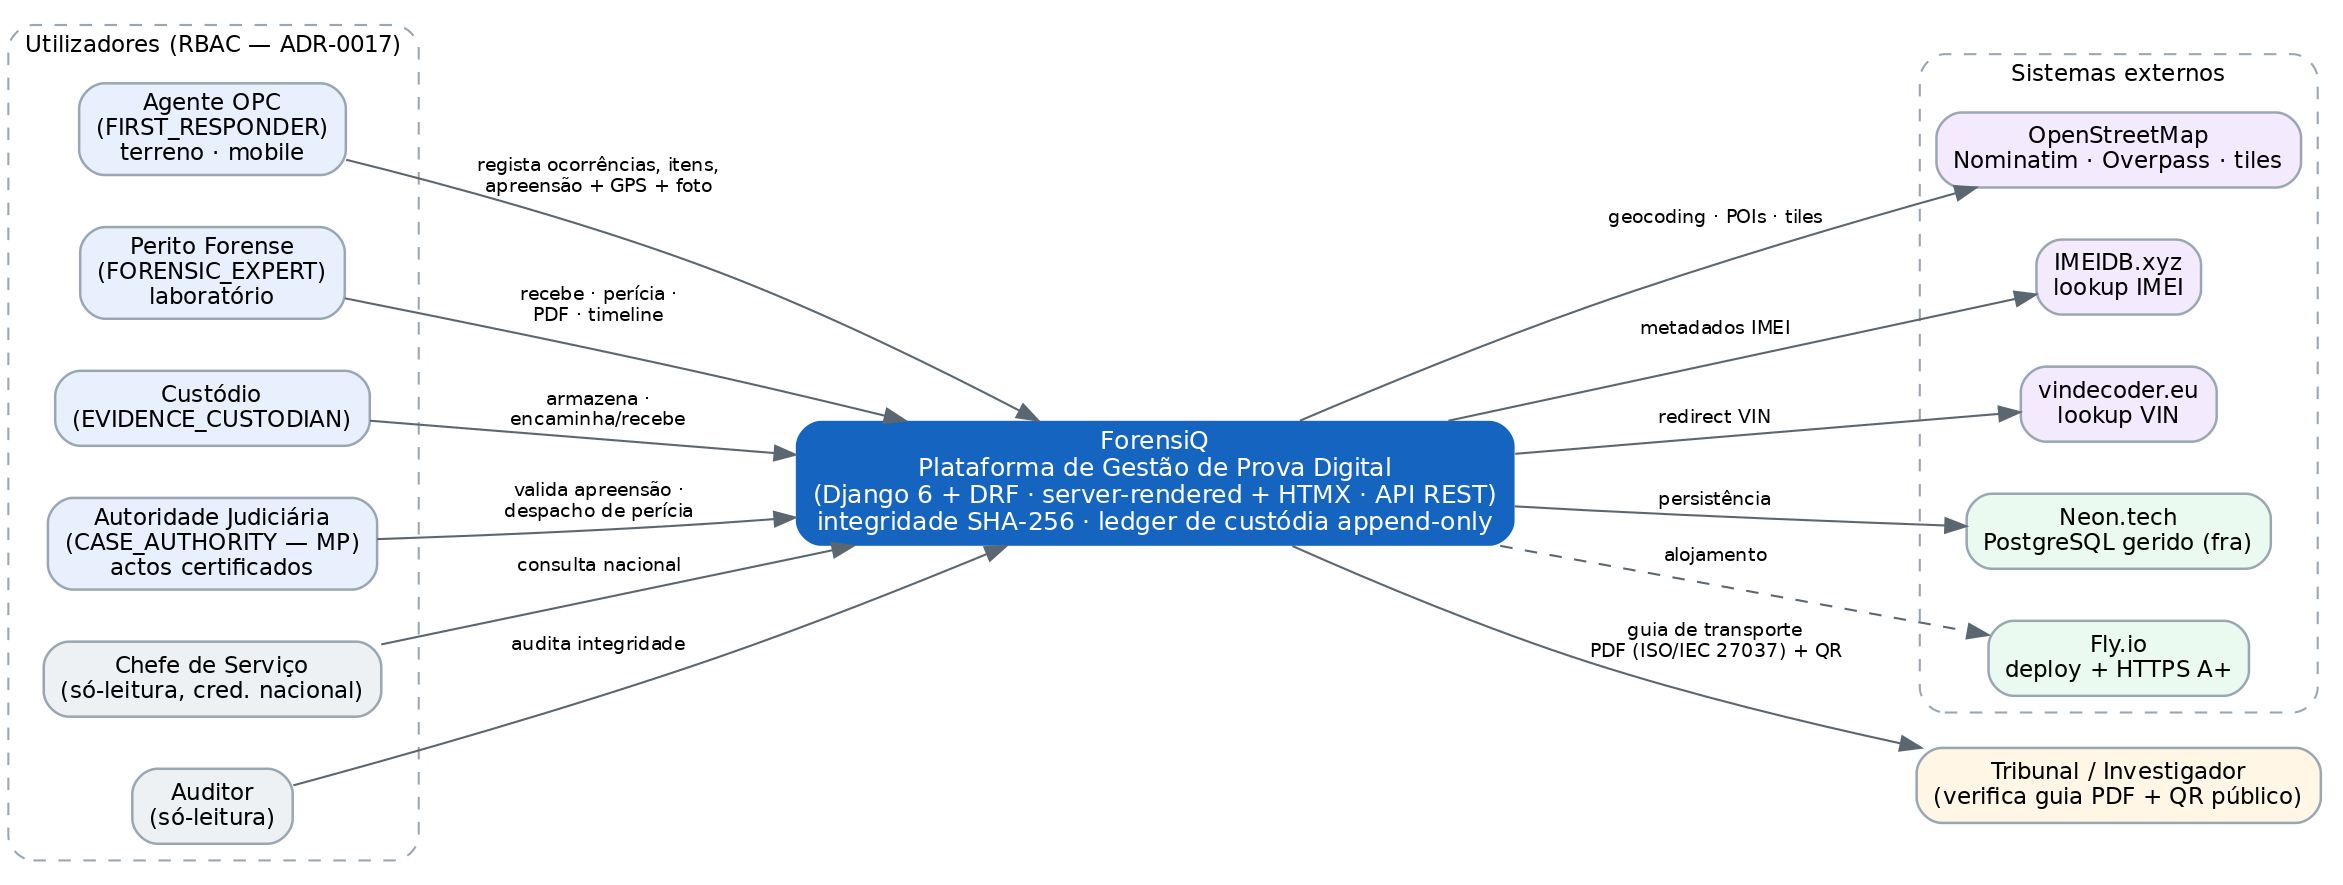
\includegraphics[width=0.85\textwidth]{c4-context.png}
\caption{Diagrama C4 nível 1: ForensiQ, utilizadores e sistemas externos.}
\label{fig:c4-l1}
\end{figure}

\subsubsection{Diagrama C4 nível 2 --- Contentores}
\label{sec:c4-l2}

A Figura~\ref{fig:c4-l2} decompõe a aplicação em três contentores
principais: a aplicação Django (servindo simultaneamente
\emph{templates} HTML e API REST), a base de dados PostgreSQL gerida
pela Neon, e o volume de \emph{media} persistente da Fly.io para
fotografias. O fonte do diagrama está em
\texttt{docs/architecture/diagrams/c4-container.mmd}.

\begin{figure}[h]
\centering
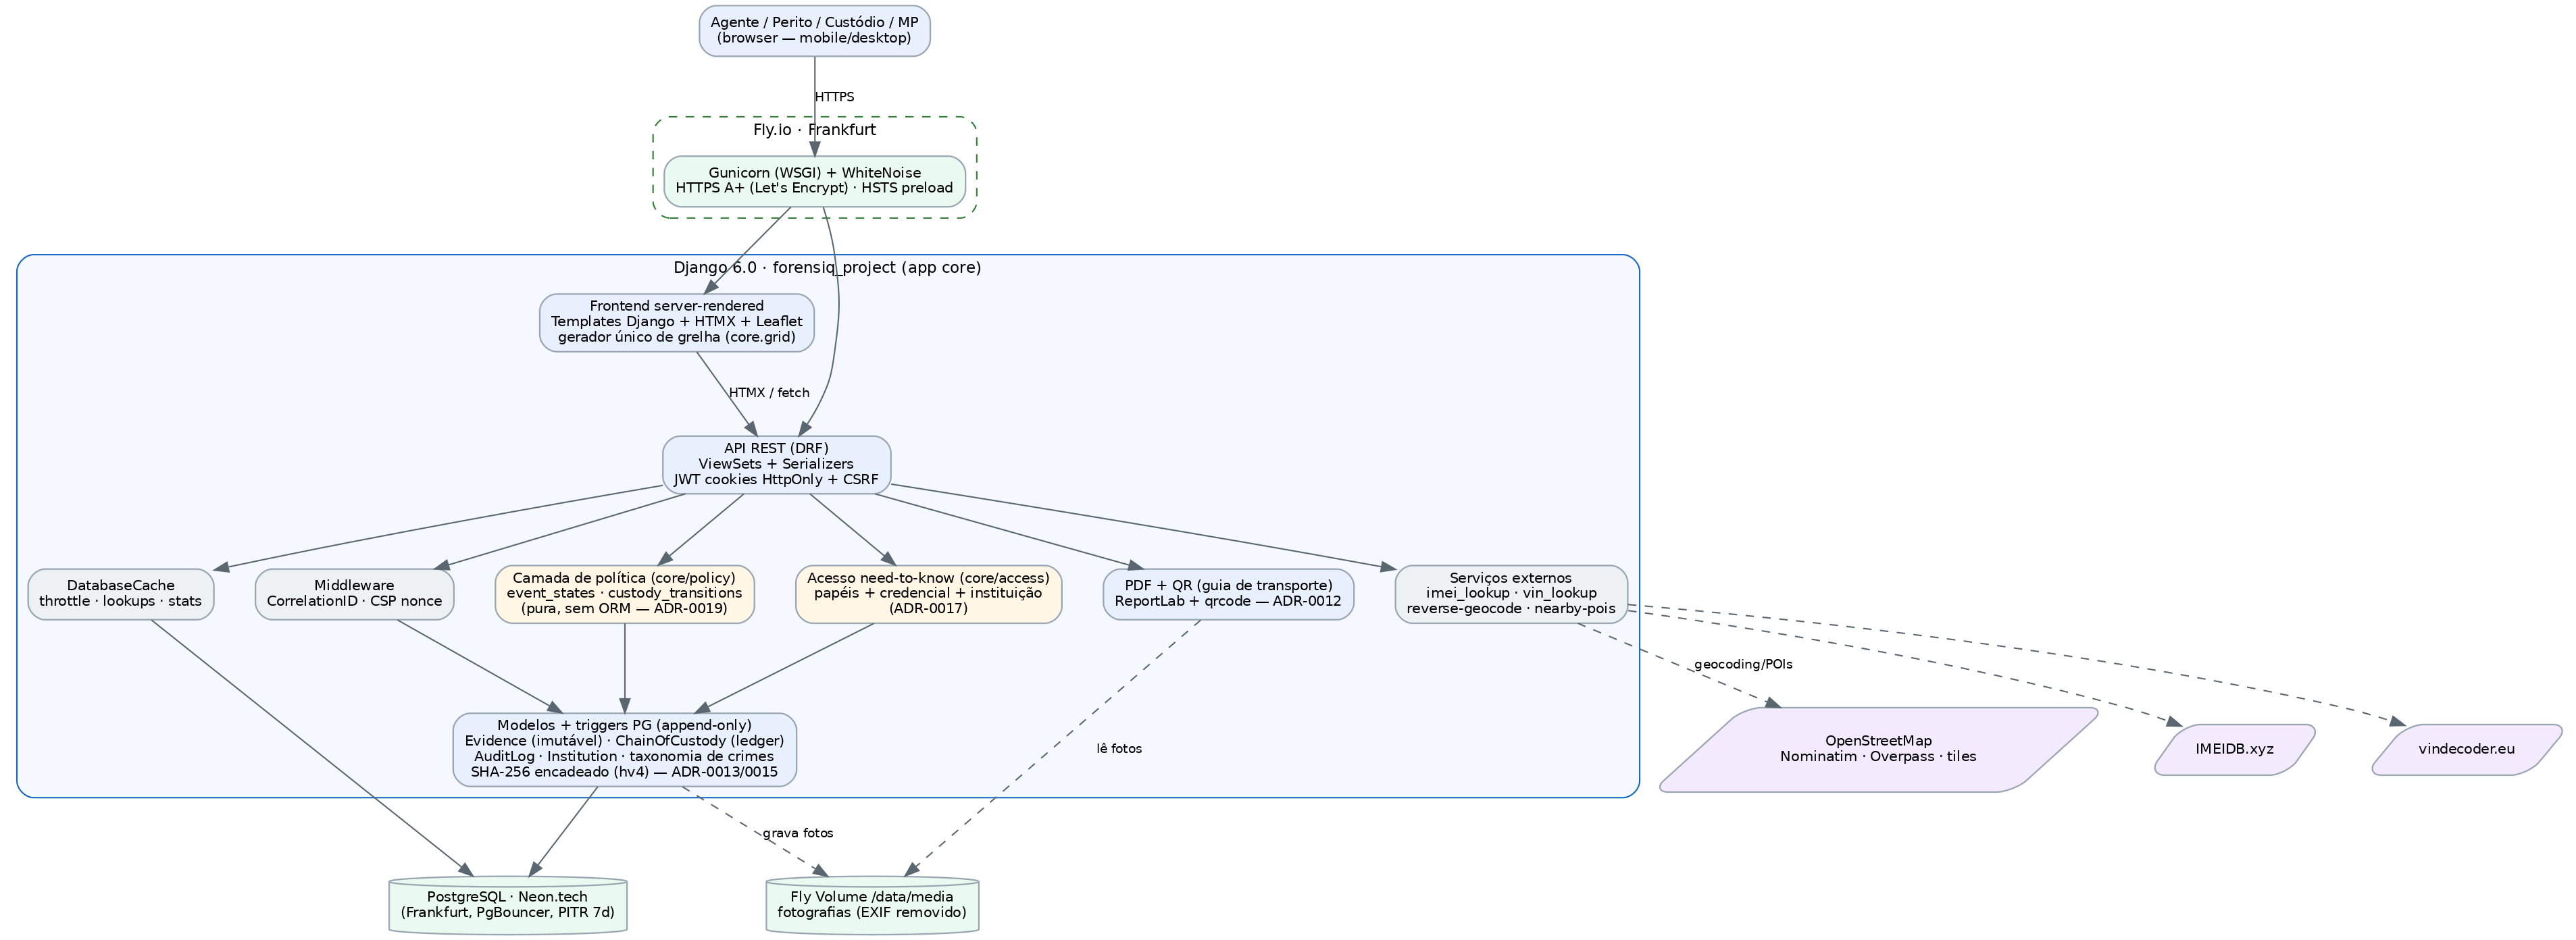
\includegraphics[width=0.95\textwidth]{c4-container.png}
\caption{Diagrama C4 nível 2 (contentores) com tecnologias principais.}
\label{fig:c4-l2}
\end{figure}

\subsubsection{Stack tecnológica}
\label{sec:stack}

A Tabela~\ref{tab:stack} resume a \emph{stack} adoptada e a
justificação sucinta de cada escolha. As decisões de fundo estão
registadas em ADRs próprios e são sumarizadas em \S\ref{sec:adrs}.

\begin{longtable}{@{}L{3.2cm}L{4.3cm}L{7.0cm}@{}}
\toprule
\textbf{Camada} & \textbf{Tecnologia} & \textbf{Motivo da escolha (ADR)} \\
\midrule
\endhead
\emph{Backend} \emph{web}              & Django 5 + DRF 3.15  & ORM maduro, \emph{admin} integrado, autenticação \emph{built-in}; \emph{ecosystem} convencional para defesa académica (ADR-0002, ADR-0003). \\
\midrule
Documentação OpenAPI                   & drf-spectacular 0.27 & Swagger~UI gerado automaticamente a partir dos \emph{viewsets}; cumpre o RF05. \\
\midrule
Autenticação                           & SimpleJWT 5 + cookies HttpOnly & JWT \emph{stateless} interoperável; transporte em \emph{cookies} mitiga XSS (ADR-0009). \\
\midrule
Validação de imagens                   & Pillow 12             & Suporte EXIF e validação MIME no \emph{upload}. \\
\midrule
Geração de PDF                         & ReportLab 4           & Geração programática conforme \emph{layout} forense, sem dependências externas. \\
\midrule
Cliente HTTP \emph{server-side}        & httpx 0.27            & Cliente moderno usado no \emph{lookup} IMEI (ADR-0008). \\
\midrule
Filtragem                              & django-filter 24      & Filtros declarativos por \emph{viewset}, integrados na API. \\
\midrule
Base de dados                          & PostgreSQL via Neon.tech & SLA gerido, \emph{branching}, \emph{point-in-time recovery} 7 dias, plano gratuito adequado ao MVP (ADR-0001). \\
\midrule
\emph{Frontend}                        & HTML5 + CSS3 + JavaScript \emph{vanilla} & Sem \emph{build step}; \emph{mobile-first}; explicabilidade total a um júri (ADR-0004). \\
\midrule
Mapa                                   & Leaflet 1.9 + OpenStreetMap & Sem chave de API; \emph{tiles} OSM com Referrer-Policy \texttt{strict-origin} (ADR-0007). \\
\midrule
Alojamento                             & Fly.io fra            & Frankfurt (próximo da Neon); HTTPS Let's Encrypt automático; volume persistente (ADR-0005). \\
\midrule
Servidor WSGI                          & Gunicorn 22 + WhiteNoise 6 & Dois \emph{workers}; estáticos servidos directamente, sem CDN. \\
\midrule
Diagramas                              & Mermaid + C4-PlantUML & \emph{Diagrams-as-code} versionados em \texttt{docs/architecture/diagrams/}. \\
\bottomrule
\caption{Pilha tecnológica do ForensiQ com justificação por camada.}\label{tab:stack}
\end{longtable}

\subsubsection{Modelo de dados}
\label{sec:datamodel}

A Figura~\ref{fig:er} apresenta o modelo entidade-relação. As entidades
centrais são \texttt{User}, \texttt{Occurrence}, \texttt{Evidence},
\texttt{DigitalDevice}, \texttt{ChainOfCustody} e \texttt{AuditLog},
todas implementadas em \texttt{src/backend/core/models.py}.

\begin{figure}[p]
\centering
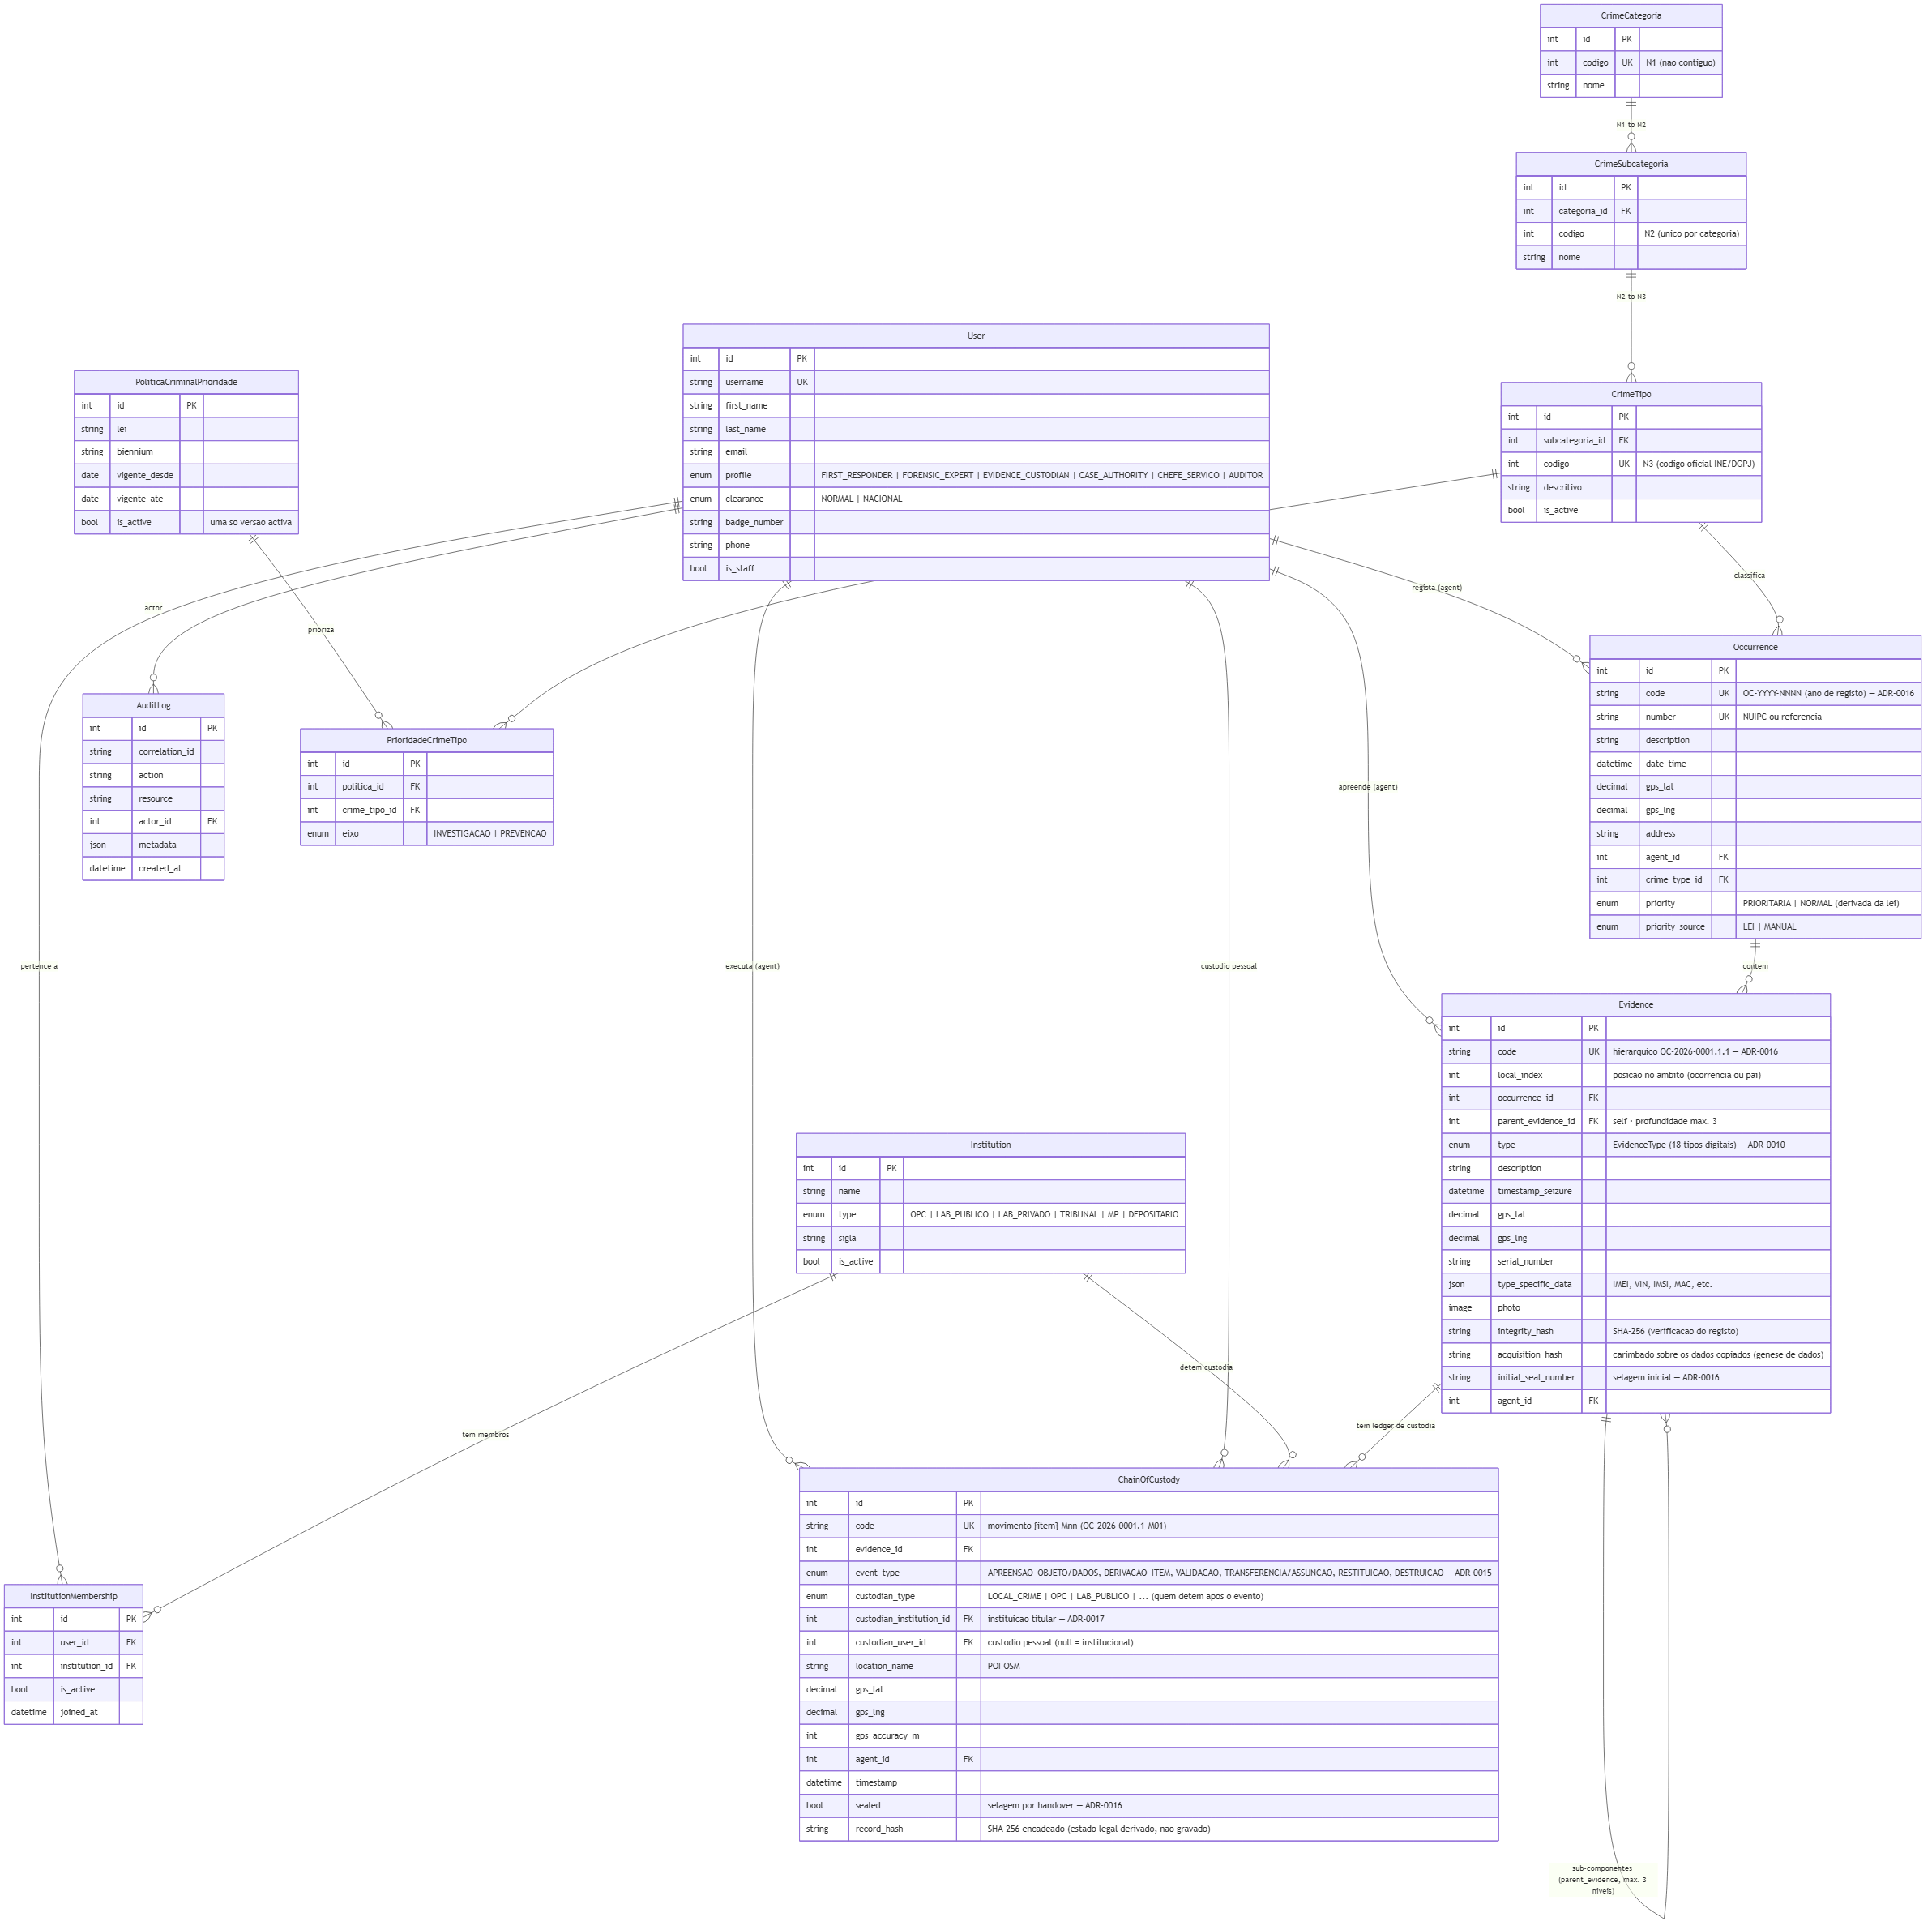
\includegraphics[height=0.92\textheight, keepaspectratio]{er-forensiq.png}
\caption{Modelo entidade-relação do ForensiQ.}
\label{fig:er}
\end{figure}

\paragraph{User} (\texttt{models.py:116--158}). Modelo Django
\texttt{AbstractUser} estendido com \texttt{profile} (escolhas
\texttt{AGENT}, \texttt{EXPERT}), \texttt{badge\_number} e
\texttt{phone}. As permissões da API consultam o \texttt{profile} via
\emph{permission classes} dedicadas em \texttt{permissions.py}.

\paragraph{Occurrence} (\texttt{models.py:164--268}). Caso ou cena
de crime, com \texttt{number} (NUIPC, formato \texttt{NUIPC.812/2026.LISBOA}),
\texttt{code} legível auto-gerado (\texttt{OCC-YYYY-NNNNN}),
\texttt{address}, coordenadas GPS, \texttt{date\_time} e \emph{foreign
key} para o agente criador.

\paragraph{Evidence} (\texttt{models.py:306--724}). Item apreendido,
com taxonomia de 18 tipos digital-first (ADR-0010): 14 raízes
(\texttt{MOBILE\_DEVICE}, \texttt{COMPUTER}, \texttt{STORAGE\_MEDIA},
\texttt{GAMING\_CONSOLE}, \texttt{GPS\_TRACKER}, \texttt{SMART\_TAG},
\texttt{CCTV\_DEVICE}, \texttt{VEHICLE}, \texttt{DRONE},
\texttt{IOT\_DEVICE}, \texttt{NETWORK\_DEVICE}, \texttt{DIGITAL\_FILE},
\texttt{RFID\_NFC\_CARD}, \texttt{OTHER\_DIGITAL}) e 4 sub-componentes
típicos (\texttt{SIM\_CARD}, \texttt{MEMORY\_CARD},
\texttt{INTERNAL\_DRIVE}, \texttt{VEHICLE\_COMPONENT}). A relação
\texttt{parent\_evidence} permite hierarquia até três níveis
(\texttt{MAX\_TREE\_DEPTH=3}, \texttt{models.py:318}); validação em
\texttt{Evidence.clean} impede ciclos e migrações entre ocorrências.
Cada evidência tem \texttt{integrity\_hash} SHA-256 calculado no
\texttt{save}, \texttt{type\_specific\_data} em \texttt{JSONField}
(com validadores dedicados de IMEI, IMSI, ICCID, MAC, VIN), fotografia
opcional, GPS e número de série.

\paragraph{DigitalDevice} (\texttt{models.py:730--851}). Ficha técnica
detalhada \emph{one-to-one} com uma \texttt{Evidence}. Coexiste com a
hierarquia de sub-componentes da \texttt{Evidence} por razões de
compatibilidade (ADR-0010).

\paragraph{ChainOfCustody} (\texttt{models.py:858--1114}). Núcleo
técnico do projecto, abordado em detalhe em \S\ref{sec:certificacao}.

\paragraph{AuditLog} (\texttt{models.py:1121--1259}). Registo
transversal de acessos e operações sensíveis: \texttt{user},
\texttt{action}, \texttt{resource\_type}, \texttt{resource\_id},
\texttt{ip\_address}, \texttt{correlation\_id} (UUID por pedido HTTP)
e \texttt{timestamp} do servidor.

\subsubsection{Decisões de arquitectura}
\label{sec:adrs}

As decisões estruturantes foram registadas como ADRs versionados em
\texttt{docs/architecture/adr/}. A Tabela~\ref{tab:adrs} sumariza as
dez decisões em vigor; o detalhe completo, com alternativas
rejeitadas, está nos ficheiros ADR.

\begin{longtable}{@{}L{1.2cm}L{4.3cm}L{9.0cm}@{}}
\toprule
\textbf{ADR} & \textbf{Tema} & \textbf{Decisão e principal alternativa rejeitada} \\
\midrule
\endhead
0001 & PostgreSQL + Neon              & Postgres com \emph{triggers} \texttt{BEFORE UPDATE/DELETE} para imutabilidade ao nível da BD; alojado na Neon free, plano \emph{Launch} antes da defesa. Rejeitadas: Supabase (pausa após 7 dias), Render (expira 30 dias), SQLite (sem \emph{triggers}). \\
\midrule
0002 & Estrutura do projecto Django   & Django 5 + DRF; \texttt{User} \texttt{AbstractUser} com \texttt{profile}; \texttt{ChainOfCustody} \emph{append-only}. Rejeitada: FastAPI (sem ORM nem \emph{admin} integrados). \\
\midrule
0003 & Desenho da API REST            & DRF \emph{ModelViewSet} + \emph{DefaultRouter}; permissões granulares por perfil; sem PUT/PATCH/DELETE em \texttt{ChainOfCustody}. \\
\midrule
0004 & Arquitectura do \emph{frontend} & HTML/CSS/JS \emph{vanilla} servido pelo Django. Rejeitada: SPA React (sobrecusto de \emph{build} e \emph{bundle}). \\
\midrule
0005 & \emph{Deployment} em produção  & Fly.io fra + Neon Postgres + IPv4 dedicado + Let's Encrypt automático. Rejeitadas: Render (sem fra; \emph{cold start}), Railway (apenas Amesterdão). \\
\midrule
0006 & Extensibilidade modular        & \emph{Apps} Django independentes para futuros módulos forenses; \emph{services layer} para \emph{hash}, exportação e auditoria. Rejeitada: herança de modelo (\emph{multi-table inheritance}). \\
\midrule
0007 & SRI e Referrer-Policy          & Manter SRI nos recursos do CDN com \emph{hashes} SHA-512 actualizados; \texttt{strict-origin-when-cross-origin}. Rejeitada: remover SRI (perde defesa em profundidade). \\
\midrule
0008 & \emph{Cache} para \emph{lookups} IMEI/VIN & \texttt{DatabaseCache} em Neon Postgres, TTL 30 dias para IMEI, 180 para VIN. Rejeitadas: \texttt{LocMemCache} (perde-se em \emph{restart}), Redis externo (custo). \\
\midrule
0009 & JWT em \emph{cookies} HttpOnly & Transporte em \texttt{fq\_access}/\texttt{fq\_refresh} HttpOnly + Secure + SameSite=Strict; CSRF \emph{double-submit}. Rejeitada: \texttt{Authorization: Bearer} em \texttt{localStorage}. \\
\midrule
0010 & Taxonomia de evidência         & 18 códigos \emph{digital-first} alinhados com ISO/IEC~27037 e ENFSI~2024; hierarquia até três níveis; \texttt{type\_specific\_data} em \texttt{JSONField}. Rejeitada: importação 1:1 da taxonomia Cellebrite UFED. \\
\bottomrule
\caption{Síntese dos dez ADRs em vigor; detalhe em \texttt{docs/architecture/adr/}.}\label{tab:adrs}
\end{longtable}

% =============================================================================
\subsection{Algoritmo de certificação e integridade}
\label{sec:certificacao}

A integridade da prova digital é o requisito mais crítico do
ForensiQ. Esta secção apresenta, do mais geral ao mais específico, o
problema adversarial, a justificação do algoritmo SHA-256, as duas
fórmulas determinísticas implementadas, o tratamento da concorrência
e a defesa em três camadas que torna a adulteração detectável mesmo
perante um atacante com acesso directo à base de dados.

\subsubsection{Modelo de ameaças aplicado}
\label{sec:threat-model}

A análise seguiu o método STRIDE simplificado para um sistema de
gestão de prova digital sem aquisição forense, sem armazenamento
distribuído e com um único \emph{tenant}. A definição operacional
adoptada de \emph{prova digital adulterada} é: qualquer registo
armazenado cujo conjunto de campos canónicos não reproduza o
\emph{hash} SHA-256 declarado, ou cuja sequência de custódia não
reproduza o encadeamento de \emph{hashes} a partir da raiz da cadeia.
A detecção é por recálculo independente, conforme ISO/IEC~27037
\S5.4--5.5~\citep{iso27037}.

\subsubsection{Escolha do algoritmo de \emph{hash}}
\label{sec:hash-choice}

A integridade dos registos forenses do ForensiQ assenta numa função
de \emph{hash} criptográfica. A norma ISO/IEC~27037 não impõe um
algoritmo específico, mas exige resistência à colisão, resistência à
pré-imagem e maturidade reconhecida. As alternativas comparadas
foram MD5 (quebrado, com colisões em segundos), SHA-1 (quebrado em
2017 com a colisão \emph{SHAttered}), SHA-3/Keccak (vigente, mas com
menos jurisprudência forense), BLAKE2/3 (rápidos, pouca adopção
forense) e SHA-256 (vigente, FIPS 180-4, sem ataques práticos
conhecidos, jurisprudência forense estabelecida). A decisão pelo
SHA-256 fundamenta-se em quatro critérios: maturidade e normalização
(FIPS 180-4 com mais de uma década), jurisprudência forense
(referência da ENFSI e da ACPO~\citep{acpo2012}), interoperabilidade
(verificável com \texttt{sha256sum} ou \texttt{certutil} em qualquer
sistema operativo, sem ferramentas especializadas), e custo
computacional desprezável para o volume previsto. A implementação
usa \texttt{hashlib.sha256} da biblioteca \emph{standard} do Python,
sem dependências de terceiros.

\subsubsection{Hash de integridade do registo de evidência}
\label{sec:integrity-hash}

Cada registo de evidência recebe, no momento da criação, um
\emph{hash} SHA-256 que cobre todos os campos canónicos mais o
conteúdo binário da fotografia anexa. A função
\texttt{compute\_integrity\_hash} (\texttt{models.py:554--584}) é
determinística e reprodutível. A Listagem~\ref{lst:integrity-hash}
apresenta a versão sintética.

\begin{lstlisting}[language=Python,caption={\texttt{compute\_integrity\_hash} (\texttt{models.py:554--584}).},label={lst:integrity-hash}]
def compute_integrity_hash(self):
    photo_hash = self._compute_photo_hash()  # SHA-256 dos bytes da imagem
    tsd_json = json.dumps(
        self.type_specific_data or {},
        sort_keys=True, separators=(',', ':'), ensure_ascii=False,
    )
    data = (
        f'{self.occurrence_id}|{self.type}|{self.parent_evidence_id or ""}|'
        f'{self.description}|{self.gps_lat}|{self.gps_lon}|'
        f'{self.timestamp_seizure.isoformat()}|{self.serial_number}|'
        f'{self.agent_id}|tsd={tsd_json}|photo={photo_hash}'
    )
    return hashlib.sha256(data.encode('utf-8')).hexdigest()
\end{lstlisting}

Três aspectos são essenciais: o \texttt{type\_specific\_data} é
serializado com \texttt{sort\_keys=True}, garantindo representação
canónica independente da ordem de inserção das chaves; a fotografia
entra na fórmula via o seu próprio \emph{hash} SHA-256
(\texttt{\_compute\_photo\_hash}, \texttt{models.py:534--552}), de
modo a que a substituição dos \emph{bytes} da imagem com manutenção
do nome do ficheiro --- vector clássico de adulteração ---
seja imediatamente detectada; o \emph{timestamp} usado é o de
apreensão (\texttt{timestamp\_seizure}), o momento forense relevante.

\subsubsection{Cadeia de custódia com \emph{hash} encadeado}
\label{sec:hash-chain}

Cada transição de estado é registada como entrada \emph{append-only}
cujo \emph{hash} SHA-256 inclui o \emph{hash} do registo anterior ---
estrutura inspirada em \emph{blockchain}, sem prova-de-trabalho. A
Figura~\ref{fig:hash-flow} apresenta o fluxo de cálculo e a
propagação da invalidação por adulteração.

\begin{figure}[h]
\centering
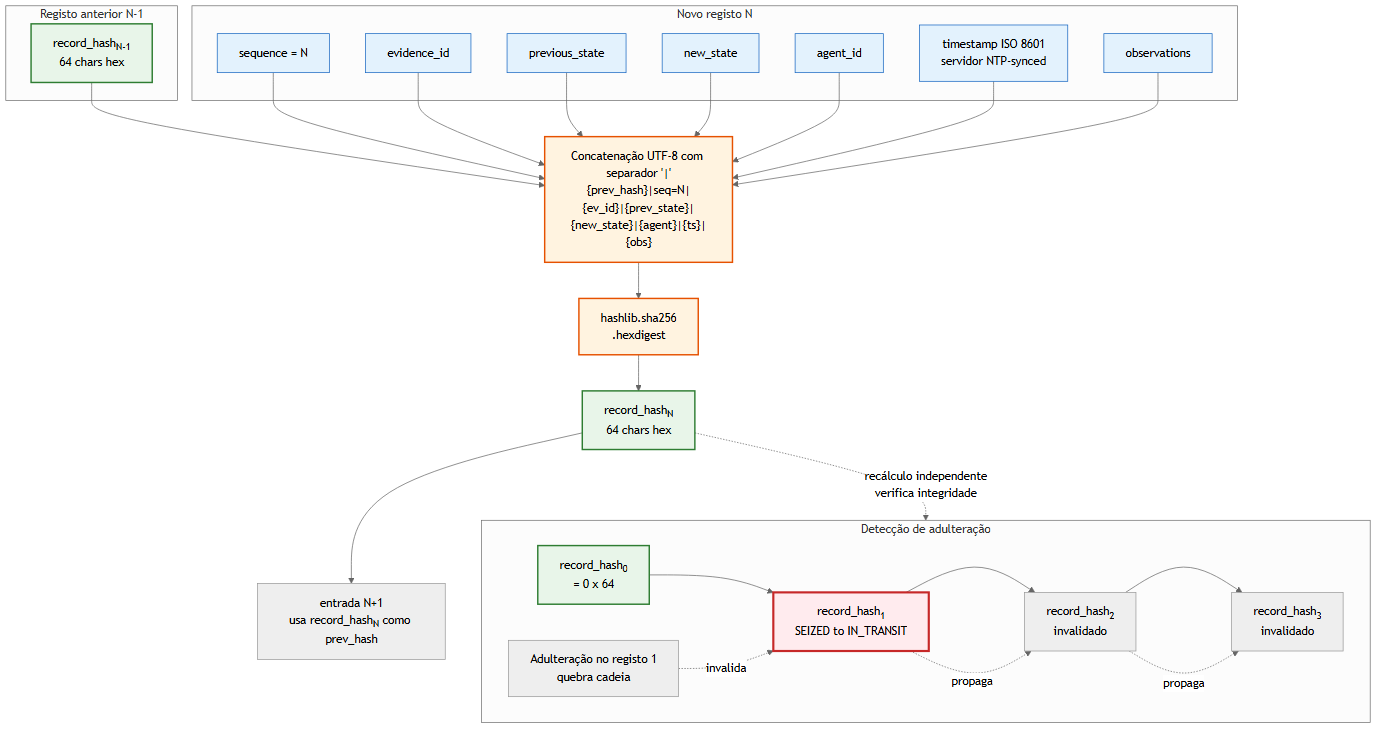
\includegraphics[width=\textwidth]{hash-chain-flow.png}
\caption{Fluxograma do cálculo do \emph{hash} encadeado e da detecção de adulteração.}
\label{fig:hash-flow}
\end{figure}

A função \texttt{compute\_record\_hash} (\texttt{models.py:989--1031})
é \emph{pura} e \emph{determinística}: recebe o \emph{hash} anterior
como parâmetro e calcula o resultado a partir exclusivamente dos
campos públicos do registo. Esta pureza permite verificabilidade
externa --- qualquer perito independente, com acesso aos campos e ao
\emph{hash} da raiz da cadeia, pode reproduzir todos os \emph{hashes}
subsequentes.

\paragraph{Fórmula canónica.}
\begin{align*}
\mathrm{record\_hash}_n = \mathrm{SHA\text{-}256}\bigl(
& \mathrm{prev\_hash}_{n-1} \mathbin{\Vert} \mathrm{seq} \mathbin{\Vert} \mathrm{evidence\_id} \\
& \mathbin{\Vert}\, \mathrm{prev\_state} \mathbin{\Vert} \mathrm{new\_state} \mathbin{\Vert} \mathrm{agent\_id} \\
& \mathbin{\Vert}\, \mathrm{ts}_{\mathrm{ISO}} \mathbin{\Vert} \mathrm{obs} \bigr)
\end{align*}

onde $\mathbin{\Vert}$ denota concatenação UTF-8 separada por
``\texttt{|}'', $\mathrm{prev\_hash}_{0} = \texttt{0} \times 64$ é
o \emph{hash} convencional da raiz, e $\mathrm{seq} = 1, 2, 3, \dots$
é o número sequencial monótono dentro da evidência, garantido por
\texttt{UniqueConstraint(evidence, sequence)}
(\texttt{models.py:957--962}).

\paragraph{Sequência canónica vs. \emph{timestamp}.}
A escolha de \texttt{sequence} (não do \emph{timestamp}) como
identificador ordinal é deliberada. \emph{Timestamps} podem sofrer
derivações entre máquinas, em particular sob dessincronização NTP, e
dois registos no mesmo segundo poderiam ambiguar a ordem. A
\texttt{UniqueConstraint(evidence, sequence)} é o invariante forense:
para cada evidência, existe no máximo um registo com cada número
sequencial.

\subsubsection{Concorrência e atomicidade}
\label{sec:concurrency}

A escrita de uma transição exige a leitura prévia do último registo
da evidência seguida da inserção do novo. Sem cuidado, esta
sequência expõe duas \emph{races}: dois agentes em escrita
concorrente podem produzir entradas com a mesma \texttt{sequence} ou
\emph{hashes} encadeados ao mesmo predecessor.

A solução combina três mecanismos PostgreSQL.
\textbf{Primeiro}, \texttt{transaction.atomic()} envolve toda a
operação numa transacção; falha em qualquer ponto reverte tudo.
\textbf{Segundo}, \texttt{select\_for\_update()} adquire um
\emph{row lock} pessimista sobre o último registo, forçando
escritores concorrentes a aguardar.
\textbf{Terceiro}, a \texttt{UniqueConstraint(evidence, sequence)}
rejeita uma sequência duplicada com \texttt{IntegrityError} mesmo
perante \emph{bug} aplicacional. A
Listagem~\ref{lst:save-atomic} apresenta o esqueleto.

\begin{lstlisting}[language=Python,caption={Inserção atómica em \texttt{ChainOfCustody.save} (\texttt{models.py:1044--1107}).},label={lst:save-atomic}]
def save(self, *args, **kwargs):
    if self.pk is not None:
        raise ValidationError('Registos imutaveis')
    with transaction.atomic():
        last_record = (
            ChainOfCustody.objects
            .select_for_update()
            .filter(evidence=self.evidence)
            .order_by('-sequence')
            .first()
        )
        self.previous_state = last_record.new_state if last_record else ''
        self.sequence = (last_record.sequence + 1) if last_record else 1
        self.timestamp = timezone.now()
        self.full_clean()
        previous_hash = last_record.record_hash if last_record else '0' * 64
        self.record_hash = self.compute_record_hash(previous_hash=previous_hash)
        super().save(*args, **kwargs)
\end{lstlisting}

A passagem explícita de \texttt{previous\_hash} a
\texttt{compute\_record\_hash} (correcção da auditoria interna de
19~abr~2026, identificada como \emph{B-C2}) elimina uma segunda
\emph{query} fora do \emph{lock}, mantendo a função \emph{pura}. O
\texttt{full\_clean()} antes do \texttt{super().save()} delega na
\texttt{ChainOfCustody.clean} (\texttt{models.py:973--987}) a
validação da transição contra \texttt{VALID\_TRANSITIONS}
(\texttt{models.py:883--892}), recusando saltos como
\texttt{APREENDIDA $\rightarrow$ EM\_PERICIA}.

\subsubsection{Imutabilidade em três camadas}
\label{sec:immutability}

A integridade de uma transição, depois de gravada, é preservada por
defesa em profundidade de três camadas independentes: ORM Django,
DRF e \emph{triggers} PostgreSQL. Cada camada presume que as
anteriores podem ter falhado ou sido contornadas. A
Figura~\ref{fig:immutability} ilustra os três caminhos de ataque
considerados.

\begin{figure}[h]
\centering
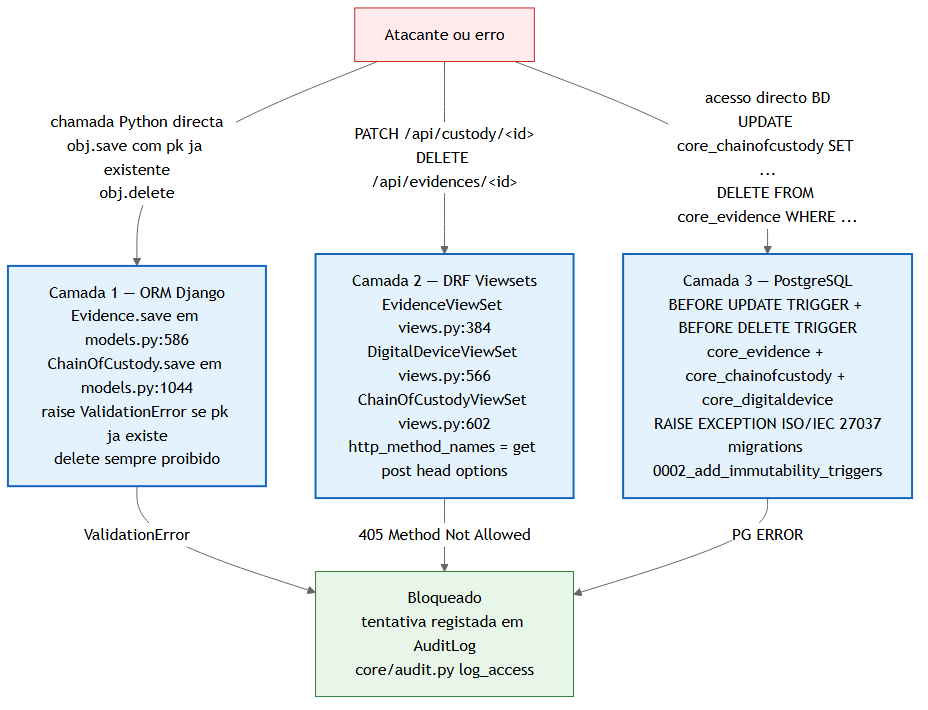
\includegraphics[width=\textwidth]{immutability-3-layers.png}
\caption{Defesa em profundidade contra adulteração: ORM, DRF e \emph{triggers} PostgreSQL.}
\label{fig:immutability}
\end{figure}

\paragraph{Camada 1 --- ORM Django.}
Os métodos \texttt{Evidence.save} (\texttt{models.py:586}),
\texttt{Evidence.delete} (\texttt{models.py:619}),
\texttt{ChainOfCustody.save} (\texttt{models.py:1044}) e
\texttt{ChainOfCustody.delete} (\texttt{models.py:1109}) interceptam
chamadas Python e lançam \texttt{ValidationError} sempre que se
detecta tentativa de actualização (\texttt{pk is not None}) ou
eliminação. Esta camada protege contra erros do próprio código
aplicacional.

\paragraph{Camada 2 --- Django REST Framework.}
\texttt{EvidenceViewSet} (\texttt{views.py:384}),
\texttt{DigitalDeviceViewSet} (\texttt{views.py:566}) e
\texttt{ChainOfCustodyViewSet} (\texttt{views.py:602}) declaram
\texttt{http\_method\_names = ['get', 'post', 'head', 'options']}; o
efeito visível para um cliente que tente \texttt{PUT}, \texttt{PATCH}
ou \texttt{DELETE} é uma resposta \texttt{405 Method Not Allowed}.

\paragraph{Camada 3 --- \emph{Triggers} PostgreSQL.}
A última linha de defesa é uma \emph{trigger} PL/pgSQL aplicada
directamente à tabela, que rejeita \texttt{UPDATE} e \texttt{DELETE}
mesmo perante \emph{queries} SQL emitidas fora da aplicação. A
Listagem~\ref{lst:trigger} é o SQL exacto, conforme
\texttt{src/backend/core/\allowbreak migrations/\allowbreak 0002\_add\_immutability\_triggers.py:63--82}.

\begin{lstlisting}[caption={\emph{Triggers} PostgreSQL em \texttt{core\_chainofcustody} (\emph{migration} \texttt{0002}).},label={lst:trigger}]
CREATE OR REPLACE FUNCTION prevent_custody_modification()
RETURNS TRIGGER AS $$
BEGIN
    RAISE EXCEPTION
        'Registos de cadeia de custodia sao imutaveis (ISO/IEC 27037). '
        'Operacao bloqueada: %', TG_OP;
END;
$$ LANGUAGE plpgsql;

CREATE TRIGGER trg_custody_no_update
    BEFORE UPDATE ON core_chainofcustody
    FOR EACH ROW EXECUTE FUNCTION prevent_custody_modification();
CREATE TRIGGER trg_custody_no_delete
    BEFORE DELETE ON core_chainofcustody
    FOR EACH ROW EXECUTE FUNCTION prevent_custody_modification();
\end{lstlisting}

A mesma \emph{migration} instala \emph{triggers} análogas para
\texttt{core\_evidence} e \texttt{core\_digitaldevice}, cobrindo as
três tabelas que materializam a prova.

% =============================================================================
\subsection{Segurança transversal}
\label{sec:security}

\subsubsection{Autenticação JWT em \emph{cookies} HttpOnly}
\label{sec:auth}

A autenticação assenta em \emph{tokens} JWT~\citep{simplejwt_docs}
transportados em \emph{cookies} \texttt{HttpOnly + Secure +
SameSite=Strict}, conforme decisão registada em ADR-0009 e
implementação em \texttt{src/backend/core/auth.py:1--90}. A escolha
do transporte por \emph{cookie} (em vez de \texttt{Authorization:
Bearer} em \texttt{localStorage}) mitiga o vector XSS: um
\emph{cookie} \texttt{HttpOnly} é opaco ao JavaScript da página, de
modo que a injecção bem-sucedida de um \emph{script} numa
vulnerabilidade de XSS não consegue exfiltrar a sessão.

Quatro detalhes são essenciais: \emph{(i)} os \emph{cookies}
\texttt{fq\_access} (validade configurável, default 60 minutos) e
\texttt{fq\_refresh} (default 7 dias) são colocados pelo
\texttt{set\_auth\_cookies} (\texttt{auth.py:71--84}) com
\texttt{httponly=True}, \texttt{secure=not settings.DEBUG} e
\texttt{samesite='Strict'}; o \emph{cookie} \texttt{csrftoken},
único não-\texttt{HttpOnly}, é o \emph{token} CSRF que o
\emph{frontend} replica em \texttt{X-CSRFToken} para pedidos
não-seguros.
\emph{(ii)} A classe \texttt{JWTCookieAuthentication}
(\texttt{auth.py:33--58}) lê o \emph{token} do cabeçalho ou, na sua
ausência, do \emph{cookie} \texttt{fq\_access}; valida-o
criptograficamente; e em pedidos com método não-seguro invoca
\texttt{enforce\_csrf} para validar \texttt{X-CSRFToken}.
\emph{(iii)} O \emph{refresh} é rotativo com \emph{blacklist}
(\texttt{ROTATE\_REFRESH\_TOKENS=True},
\texttt{BLACKLIST\_AFTER\_ROTATION=True} em \texttt{settings.py:180--181}),
reduzindo a janela de exploração em caso de roubo.
\emph{(iv)} Os três \emph{endpoints} de autenticação têm
\texttt{AuthRateThrottle} de cinco pedidos por minuto, configurado
em \texttt{REST\_FRAMEWORK['DEFAULT\_THROTTLE\_RATES']}, para travar
força bruta.

\subsubsection{Autorização baseada em papéis (RBAC)}
\label{sec:rbac}

O modelo de autorização é granular por papel e por recurso, conforme
ADR-0003. Existem dois papéis operacionais (\texttt{AGENT} e
\texttt{EXPERT}, em \texttt{User.profile}) mais a \emph{flag}
\texttt{is\_staff} para administração. Cinco classes de permissão
implementadas em \texttt{src/backend/core/permissions.py}:
\texttt{IsAgent}, \texttt{IsExpert}, \texttt{IsAgentOrExpert},
\texttt{IsOwnerOrReadOnly} e a classe-padrão \texttt{IsAuthenticated}
do DRF.

A protecção contra IDOR (\emph{Insecure Direct Object Reference}) é
adicional: o \texttt{get\_queryset()} de cada \emph{viewset} restringe
os recursos ao utilizador autenticado quando o perfil é
\texttt{AGENT}; a classe \texttt{IsOwnerOrReadOnly} valida
\emph{ownership} em escritas. O conjunto \texttt{AuthorizationIDORTest}
em \texttt{tests\_api.py} exercita o caminho cruzado agente A
\emph{vs.}\ agente B.

\subsubsection{Cabeçalhos HTTP de segurança}
\label{sec:http-headers}

A defesa em camada HTTP combina \emph{settings} Django (em
produção, \texttt{DEBUG=False}) e o \emph{middleware} dedicado
\texttt{ContentSecurityPolicyMiddleware}
(\texttt{middleware.py:68--155}). Os controlos principais são:

\begin{itemize}[leftmargin=2em]
    \item \texttt{Strict-Transport-Security} (HSTS) com
          \texttt{max-age=31536000} (um ano), \texttt{includeSubDomains}
          e \texttt{preload} (\texttt{settings.py:284--286}). O domínio
          \texttt{forensiq.pt} foi submetido à lista \emph{preload} dos
          principais \emph{browsers} (validação externa em
          \S\ref{sec:external-tests}).
    \item \texttt{Content-Security-Policy} de nível 3, gerada por
          pedido. \texttt{default-src 'self'};
          \texttt{script-src 'self' 'nonce-\{nonce\}' https://cdnjs.cloudflare.com}
          (sem \texttt{unsafe-inline});
          \texttt{style-src 'self' 'nonce-\{nonce\}' cdnjs fonts.googleapis};
          \texttt{frame-ancestors 'none'};
          \texttt{upgrade-insecure-requests}. O \emph{nonce} é único
          por pedido (\texttt{secrets.token\_urlsafe(16)}).
    \item \texttt{Referrer-Policy: strict-origin-when-cross-origin}
          (ADR-0007) --- envia apenas a origem em pedidos
          \emph{cross-origin}, satisfazendo a política do
          OpenStreetMap sem expor \emph{paths} internos.
    \item \texttt{X-Content-Type-Options: nosniff},
          \texttt{Cross-Origin-Opener-Policy: same-origin},
          \texttt{Cross-Origin-Resource-Policy: same-origin} e
          \texttt{Permissions-Policy} restritiva.
    \item \emph{Subresource Integrity} (SRI) SHA-512 nos recursos
          do CDN da Cloudflare (Leaflet 1.9.4), declarado em
          \texttt{\_leaflet\_head.html} e \texttt{\_leaflet\_js.html}
          (ADR-0007).
\end{itemize}

\subsubsection{Outras defesas}
\label{sec:other-defenses}

\textbf{Limitação de débito} via \texttt{DEFAULT\_THROTTLE\_RATES}:
\texttt{anon} 10/min, \texttt{user} 60/min, \texttt{auth} 5/min,
\texttt{evidence\_upload} 20/min, \texttt{pdf\_export} 30/min,
\texttt{csv\_export} 10/min, \texttt{schema} 30/min
(\texttt{settings.py:142--150}). \textbf{Paginação obrigatória} via
\texttt{BoundedPageNumberPagination} (default 50, máximo 100,
\texttt{pagination.py}). \textbf{Ocultação do \emph{Django Admin}}
por prefixo configurável em \texttt{ADMIN\_URL\_PREFIX}; é segurança
por obscuridade que complementa, não substitui, a autenticação.

% =============================================================================
\subsection{Conformidade ISO/IEC 27037 e RGPD Art.~32}
\label{sec:compliance}

\subsubsection{Mapeamento à norma ISO/IEC 27037:2012}
\label{sec:iso27037}

A norma ISO/IEC~27037:2012~\citep{iso27037} estabelece princípios
e controlos para a identificação, recolha, aquisição e preservação
de prova digital. A Tabela~\ref{tab:iso} resume o mapeamento entre
as secções relevantes da norma e os mecanismos do ForensiQ; o
documento completo de rastreabilidade está em
\texttt{docs/scope/iso27037-traceability.tex}~v1.2 (3~mai~2026).

\begin{longtable}{@{}L{1.6cm}L{4.8cm}L{8.2cm}@{}}
\toprule
\textbf{Secção} & \textbf{Princípio da norma} & \textbf{Implementação no ForensiQ} \\
\midrule
\endhead
\S5.1 & Princípios gerais; integridade, auditabilidade & RBAC com perfis \texttt{AGENT}/\texttt{EXPERT} (\S\ref{sec:rbac}); JWT rotativo (\S\ref{sec:auth}); \texttt{AuditLog} com \texttt{correlation\_id}. \\
\midrule
\S5.2 & Identificação de prova digital & \texttt{Evidence} com 18 tipos digital-first (ADR-0010), descrição, \texttt{serial\_number}, GPS, \emph{timestamp} de apreensão, \emph{hash}. \\
\midrule
\S5.3 & Recolha e aquisição & \texttt{integrity\_hash} cobre metadados \emph{e bytes} da fotografia (\S\ref{sec:integrity-hash}); GPS no \emph{frontend} via \emph{Geolocation API}. \\
\midrule
\S5.4 & Preservação de integridade (3 camadas) & \emph{Append-only} no ORM (\S\ref{sec:immutability}); \emph{viewsets} com \texttt{http\_method\_names} restrito; \emph{triggers} PostgreSQL na \emph{migration} 0002. \\
\midrule
\S5.5 & Cadeia de custódia & Máquina de estados linear de 7 estados PT (\S\ref{sec:state-machine}); \emph{record\_hash} encadeado (\S\ref{sec:hash-chain}). \\
\midrule
\S6.1--6.2 & Competência e documentação & RBAC fino; PDF forense gerado por \texttt{pdf\_export.py} com declaração ISO/IEC~27037 incorporada. \\
\midrule
\S7.1--7.2 & Dispositivos e suportes & \texttt{DigitalDevice} (ficha técnica) e taxonomia detalhada de suportes em \texttt{Evidence.type}; campos específicos via \texttt{type\_specific\_data} (JSON determinístico). \\
\bottomrule
\caption{Mapeamento sintético da ISO/IEC~27037:2012 aos mecanismos do ForensiQ.}
\label{tab:iso}
\end{longtable}

\subsubsection{Conformidade com o RGPD Art.~32}
\label{sec:rgpd}

O Artigo~32.\textordfeminine{} do RGPD~\citep{rgpd2016} exige
medidas técnicas e organizacionais adequadas ao risco. A
Tabela~\ref{tab:rgpd} apresenta o sumário executivo, com identificação
honesta das lacunas relevantes; o tratamento detalhado está em
\texttt{docs/compliance/rgpd-art32-checklist.md}.

\begin{longtable}{@{}cL{4.5cm}L{2cm}L{6.5cm}@{}}
\toprule
\textbf{Alínea} & \textbf{Domínio} & \textbf{Estado} & \textbf{Lacunas a endereçar} \\
\midrule
\endhead
a) & Pseudonimização e cifragem        & Parcial         & \texttt{media/} sem cifra ao nível da aplicação. \\
\midrule
b) & CIA-R                              & Parcial         & Validação a generalizar a todos os modelos. \\
\midrule
c) & Restabelecimento de acesso         & \emph{Não conforme} & Sem \emph{backups} de \texttt{media/}; sem RTO/RPO formais. \\
\midrule
d) & Avaliação regular da eficácia      & Parcial         & Sem SAST/DAST/SCA em \emph{pipeline} CI; sem \emph{pentest} externo formal. \\
\bottomrule
\caption{Sumário executivo da conformidade RGPD Art.~32.}
\label{tab:rgpd}
\end{longtable}

A leitura honesta deste mapeamento é a seguinte: o ForensiQ tem
posicionados os controlos correctos em CIA, integridade e
auditoria, mas não está em condições de operar com dados reais sem
que as lacunas das alíneas~c) e~d) sejam endereçadas. Esta posição
é defensável em contexto académico e a sua identificação explícita
é parte da contribuição do projecto.

\subsubsection{Evidência externa de postura de segurança}
\label{sec:external-tests}

Três serviços externos independentes auditaram a postura de
segurança do ambiente de produção em
\href{https://forensiq.pt}{forensiq.pt} a 18 de Abril de 2026. Os
relatórios completos estão em
\texttt{docs/compliance/external-tests/}.

\begin{table}[h]
\centering\small
\begin{tabular}{@{}L{4.5cm}L{4.0cm}L{4.5cm}@{}}
\toprule
\textbf{Teste} & \textbf{Serviço} & \textbf{Resultado} \\
\midrule
\emph{HSTS Preload Submission} & hstspreload.org (Chromium / Mozilla / Edge / Apple) & Submetido para inclusão na lista pré-carregada \\
\emph{HTTP Observatory}        & Mozilla & Pontuação A+ (CSP, HSTS, Referrer-Policy, X-Content-Type-Options) \\
\emph{SSL Server Test}         & Qualys SSL Labs & Grau A+ (TLS 1.2/1.3, ECDHE, HSTS, OCSP \emph{stapling}) \\
\bottomrule
\end{tabular}
\caption{Resultado dos três testes externos de segurança (18~Abr 2026).}
\label{tab:external}
\end{table}

A submissão à lista \emph{HSTS preload} satisfaz o requisito
funcional adicional de HTTPS estrito mesmo no primeiro acesso (sem
janela de \emph{trust on first use}), o que é particularmente
relevante para um sistema que circula prova judicial.

% =============================================================================
\subsection{Interface do utilizador}
\label{sec:ui}

\subsubsection{Princípios de desenho}
\label{sec:ui-principles}

A \emph{interface} foi desenhada \emph{mobile-first}, conforme
ADR-0004, e respeita as Web Content Accessibility Guidelines~2.1
nível~AA. As decisões foram orientadas pelo contexto operacional do
agente: utilização com uma só mão, alvos tácteis de pelo menos
$48 \times 48$ pixéis, contraste mínimo de $4{:}5$ para texto
não-decorativo, \emph{focus rings} consistentes, \texttt{aria-busy}
em listas dinâmicas, \texttt{aria-pressed} em \emph{toggles} e
\emph{live regions} para anúncios. O sistema de cores inclui
\emph{tokens} semânticos por estado de custódia
(\texttt{--state-apreendida}, \texttt{--state-em-pericia}, etc.). A
tipografia combina \emph{Inter} para texto e \emph{JetBrains Mono}
para identificadores hexadecimais (\emph{hashes}, IDs e
\emph{timestamps}). O modo claro e o modo escuro são alternáveis e
activam-se automaticamente uma hora após o pôr do sol no local
actual, calculado em \emph{client-side} a partir da posição GPS e da
fórmula NOAA (\texttt{settings.js:145--189}).

\subsubsection{Vistas-chave}
\label{sec:ui-views}

A aplicação organiza-se em torno de treze vistas principais,
servidas por \emph{templates} em \texttt{src/frontend/templates/}:
autenticação (\texttt{/login/}); \emph{dashboard} com saudação,
acções rápidas e estatísticas por estado de custódia
(\texttt{/dashboard/}); listagem e mapa de ocorrências
(\texttt{/occurrences/}); criação de ocorrência por \emph{wizard}
(\texttt{/occurrences/new/}); \emph{hub} da ocorrência
(\texttt{/occurrences/<id>/}); listagem de evidências
(\texttt{/evidences/}); \emph{wizard} de evidência com captura de
fotografia, GPS, \emph{lookup} IMEI/VIN e sub-componentes
(\texttt{/evidences/new/}); detalhe da evidência
(\texttt{/evidences/<id>/}); \emph{timeline} de custódia
(\texttt{/evidences/<id>/custody/}); listagem de transições
(\texttt{/custodies/}); estatísticas agregadas (\texttt{/stats/});
relatórios PDF (\texttt{/reports/}); definições de perfil e tema
(\texttt{/settings/}).

\subsubsection{Wizard de evidência}
\label{sec:wizard}

O \emph{wizard} de criação de evidência é a \emph{interface}
principal de captura no terreno e está implementado em
\texttt{src/frontend/templates/evidences\_new.html:40--289} com
oito passos sequenciais: (1)~selecção da ocorrência; (2)~tipo da
evidência, com selector visual agrupado pelas duas grandes famílias
(raízes e sub-componentes); (3)~descrição livre; (4)~data e hora de
apreensão (preenchidas por omissão com o servidor);
(5)~detalhes específicos do tipo (\emph{e.g.} IMEI para
\texttt{MOBILE\_DEVICE}, com botão de \emph{lookup} externo);
(6)~fotografia (câmara nativa via atributo \texttt{capture="environment"}
ou \emph{upload} de ficheiro);
(7)~GPS (\emph{Geolocation API} do \emph{browser} + geocodificação
inversa Nominatim em PT); (8)~resumo com revisão completa antes da
submissão.

\subsubsection{Máquina de estados de custódia}
\label{sec:state-machine}

A máquina de estados que governa a vida da prova é \emph{linear} e
sem retrocesso, com dois estados terminais. A
Figura~\ref{fig:state-machine} apresenta o autómato; a sua
implementação no dicionário \texttt{ChainOfCustody.VALID\_TRANSITIONS}
(\texttt{models.py:883--892}) foi já discutida em
\S\ref{sec:concurrency}.

\begin{sidewaysfigure}
\centering
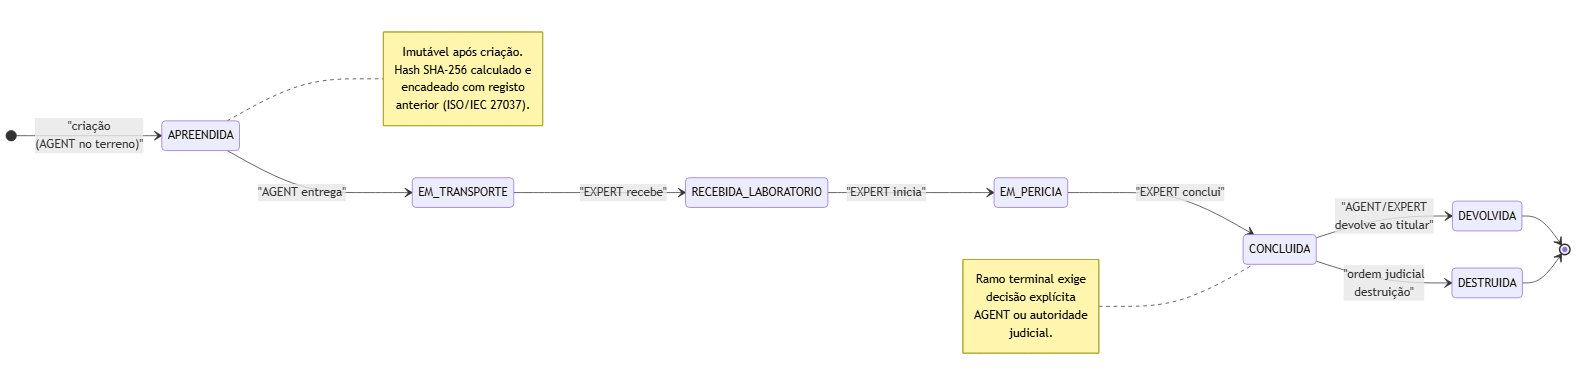
\includegraphics[width=0.95\textheight, height=0.85\textwidth, keepaspectratio]{state-machine-custody.png}
\caption{Máquina de estados da cadeia de custódia. Transições válidas a partir de cada estado; \texttt{DEVOLVIDA} e \texttt{DESTRUIDA} são terminais.}
\label{fig:state-machine}
\end{sidewaysfigure}

A transição inicial $\emptyset \rightarrow \texttt{APREENDIDA}$ é
a única origem possível para uma evidência recém-registada; a
partir daí o caminho canónico segue \texttt{APREENDIDA $\rightarrow$
EM\_TRANSPORTE $\rightarrow$ RECEBIDA\_LABORATORIO $\rightarrow$
EM\_PERICIA $\rightarrow$ CONCLUIDA}, terminando em
\texttt{DEVOLVIDA} ou \texttt{DESTRUIDA} consoante o destino
judicial.

% =============================================================================
% Cap. 3 — Implementação (estado actual à data do intercalar, conforme guia §3)
% =============================================================================

\section{Implementação --- Estado actual}
\label{cap:implementacao}

Este capítulo documenta o estado de implementação à data deste
relatório intercalar (3~de~Maio~de~2026), apresentando a
decomposição de tarefas com precedências (\S\ref{sec:tasks}), o
estado por componente (\S\ref{sec:components}), o cumprimento dos
critérios de aceitação (\S\ref{sec:acceptance}), os desvios ao plano
(\S\ref{sec:deviations}) --- incluindo o reconhecimento honesto da
demo interna síncrona não realizada na janela prevista ---,
a demonstração em produção (\S\ref{sec:demo}), o estado dos testes
automatizados (\S\ref{sec:tests-state}) e o calendário actualizado
para a fase restante (\S\ref{sec:calendario-restante}).

\subsection{Decomposição do trabalho}
\label{sec:tasks}

O trabalho foi decomposto em onze tarefas principais com precedências
implícitas, conforme a Tabela~\ref{tab:tasks}.

\begin{longtable}{@{}cL{6.0cm}L{4.5cm}L{2.0cm}@{}}
\toprule
\textbf{T} & \textbf{Tarefa} & \textbf{Precedências} & \textbf{Estado} \\
\midrule
\endhead
T1  & Configuração do repositório, proposta e MoSCoW            & ---       & Concluída \\
T2  & ADRs 0001--0010 com alternativas consideradas             & T1        & Concluída \\
T3  & Modelo de dados core                                      & T2        & Concluída \\
T4  & Autenticação JWT em \emph{cookies} HttpOnly + CSRF        & T3        & Concluída \\
T5  & API REST e \emph{viewsets}                                & T3, T4    & Concluída \\
T6  & \emph{Frontend} \emph{vanilla} \emph{mobile-first}        & T5        & Concluída \\
T7  & Imutabilidade tripla (ORM, DRF, \emph{triggers} PG)       & T3, T5    & Concluída \\
T8  & Auditoria interna de segurança e correcções               & T7        & Concluída \\
T9  & \emph{Deployment} Fly.io + Neon; HSTS \emph{preload}      & T6        & Concluída \\
T10 & \emph{Wizard} de evidência, \emph{lookups}, exportação PDF & T5, T6   & Concluída \\
T11 & Relatório intercalar                                      & T1--T10   & Em curso \\
\bottomrule
\caption{Decomposição de tarefas com precedências.}
\label{tab:tasks}
\end{longtable}

\subsection{Estado final por componente}
\label{sec:components}

A Tabela~\ref{tab:components} resume o estado de cada componente. O
estado verde indica conclusão validada por testes; amarelo indica
funcionalidade entregue com limitação reconhecida; vermelho indica
funcionalidade fora do âmbito do MVP ou ainda em curso.

\begin{longtable}{@{}L{4cm}L{2cm}L{8cm}@{}}
\toprule
\textbf{Componente} & \textbf{Estado} & \textbf{Observação} \\
\midrule
\endhead
\emph{Backend} Django + DRF                  & \cellcolor{green!12}\textcolor{successgreen}{verde}  & 213 testes a passar; modelos, \emph{viewsets}, serializadores, permissões. \\
\midrule
Cadeia de custódia (SHA-256 encadeado)       & \cellcolor{green!12}\textcolor{successgreen}{verde}  & \texttt{transaction.atomic} + \texttt{select\_for\_update} (correcções da auditoria interna). \\
\midrule
Imutabilidade tripla                         & \cellcolor{green!12}\textcolor{successgreen}{verde}  & ORM + DRF + \emph{triggers} PostgreSQL (\emph{migration} 0002). \\
\midrule
Autenticação JWT em \emph{cookies}           & \cellcolor{green!12}\textcolor{successgreen}{verde}  & HttpOnly + Secure + SameSite=Strict; CSRF \emph{double-submit}; \emph{rate limit} 5/min. \\
\midrule
\emph{Frontend} \emph{vanilla}               & \cellcolor{green!12}\textcolor{successgreen}{verde}  & 13 vistas \emph{mobile-first}; sem \emph{build step}; tema dia/noite com sunset NOAA. \\
\midrule
Mapa Leaflet + OpenStreetMap                 & \cellcolor{green!12}\textcolor{successgreen}{verde}  & Leaflet 1.9.4 com SRI SHA-512; Referrer-Policy \texttt{strict-origin-when-cross-origin}. \\
\midrule
Exportação PDF (RF6)                         & \cellcolor{green!12}\textcolor{successgreen}{verde}  & ReportLab; \texttt{/api/evidences/<id>/pdf/} e \texttt{/api/occurrences/<id>/pdf/} com declaração ISO/IEC~27037. \\
\midrule
Exportação CSV                               & \cellcolor{green!12}\textcolor{successgreen}{verde}  & \emph{Streaming} com \emph{cap} de 10 000 linhas; respeita \emph{ownership}; \emph{audit log} regista cada exportação. \\
\midrule
Lookup IMEI/VIN                              & \cellcolor{green!12}\textcolor{successgreen}{verde}  & \texttt{DatabaseCache} 30 dias (IMEI) e 180 dias (VIN). \\
\midrule
\emph{Deployment}                            & \cellcolor{green!12}\textcolor{successgreen}{verde}  & Fly.io fra + Neon; HTTPS A+ (Qualys); HSTS \emph{preload} submetido; Mozilla Observatory A+. \\
\midrule
Cobertura de testes                          & \cellcolor{orange!15}\textcolor{warningorange}{amarelo} & 67{,}4\% global; áreas com cobertura insuficiente reconhecidas (\texttt{validators.py}, \texttt{imei\_lookup.py}, \texttt{seed\_demo.py}). \\
\midrule
\emph{Backups} de \texttt{media/}            & \cellcolor{red!15}\textcolor{dangerred}{vermelho}    & Volume Fly.io persistente sem \emph{backup} externo automatizado; trabalho futuro. \\
\midrule
SAST/SCA/DAST em CI                          & \cellcolor{red!15}\textcolor{dangerred}{vermelho}    & Fora do âmbito do MVP; documentado para Fase~3. \\
\bottomrule
\caption{Estado por componente à data do intercalar.}
\label{tab:components}
\end{longtable}

\subsection{Cumprimento dos critérios de aceitação}
\label{sec:acceptance}

A Tabela~\ref{tab:acceptance} confronta o estado dos requisitos
funcionais (RF) e não-funcionais (RNF) inscritos em
\texttt{docs/scope/requirements.tex} (v1.0) com a sua verificação
empírica à data deste intercalar. Os requisitos \emph{Must have}
foram todos cumpridos. Os \emph{Should have} foram cumpridos. Os
\emph{Could have} estão parcialmente cumpridos. Os \emph{Won't have}
permaneceram fora do âmbito.

\begin{longtable}{@{}cL{8.5cm}L{2.0cm}L{2.5cm}@{}}
\toprule
\textbf{ID} & \textbf{Requisito} & \textbf{Prioridade} & \textbf{Estado} \\
\midrule
\endhead
RF01 & Autenticação JWT com perfis                       & Must  & \cellcolor{green!12}Cumprido \\
RF02 & Ocorrências com georreferenciação                 & Must  & \cellcolor{green!12}Cumprido \\
RF03 & Registo de prova com foto, GPS, \emph{hash}       & Must  & \cellcolor{green!12}Cumprido \\
RF04 & Ficha de dispositivo digital                       & Must  & \cellcolor{green!12}Cumprido \\
RF05 & Cadeia de custódia \emph{append-only} encadeada    & Must  & \cellcolor{green!12}Cumprido \\
RF06 & Exportação PDF                                     & Must  & \cellcolor{green!12}Cumprido \\
RF07 & API REST com 10+ \emph{endpoints} documentados     & Must  & \cellcolor{green!12}Cumprido (mais de 12 \emph{endpoints}) \\
RF08 & \emph{Dashboard} por estado                        & Should & \cellcolor{green!12}Cumprido \\
RF09 & Pesquisa e filtragem                               & Should & \cellcolor{green!12}Cumprido \\
RF10 & Perfis adicionais (coordenador, magistrado)        & Could & \cellcolor{orange!15}Estrutura preparada (ADR-0006) \\
RF11 & Verificação de IMEI via \emph{API} externa         & Could & \cellcolor{green!12}Cumprido (ADR-0008) \\
RF12 & \emph{Dashboard} analítico                         & Could & \cellcolor{green!12}Cumprido (\texttt{/stats/}) \\
RF13 & Despachos judiciais                                & Could & \cellcolor{red!15}Não realizado \\
RF14--RF17 & Integração PSP, dados reais, módulos QBF, \emph{app} nativa & Won't & \cellcolor{gray!15}Fora do âmbito \\
\midrule
RNF01 & HTTPS obrigatório                                 & Must  & \cellcolor{green!12}Cumprido (HSTS \emph{preload} + Qualys A+) \\
RNF02 & \emph{Mobile-first} utilizável com uma só mão      & Must  & \cellcolor{green!12}Cumprido (WCAG 2.1 AA) \\
RNF03 & Integridade SHA-256 e \emph{append-only}           & Must  & \cellcolor{green!12}Cumprido \\
RNF04 & Resposta inferior a 2 s                           & Should & \cellcolor{green!12}Verificado em produção \\
RNF05 & Testes automatizados em módulos críticos           & Should & \cellcolor{green!12}213 testes a passar \\
RNF06 & \emph{Deployment} público                         & Could & \cellcolor{green!12}\href{https://forensiq.pt}{forensiq.pt} \\
\bottomrule
\caption{Cumprimento dos requisitos funcionais e não-funcionais.}
\label{tab:acceptance}
\end{longtable}

\subsection{Desvios ao plano}
\label{sec:deviations}

A execução afastou-se em três pontos do plano apresentado na
proposta; todos foram comunicados ao orientador.

\paragraph{\emph{Stack} do \emph{backend}.}
A proposta indicava \emph{``Django + DRF''} como opção principal,
sem alternativa. A escolha foi confirmada em ADR-0002 e mantida.
Sem desvio.

\paragraph{Demo interna síncrona não realizada na janela prevista
(Sem.~7).}
O calendário do orientador previa demo interna síncrona via Teams
entre 28~de~Abril e 2~de~Maio de 2026 (Sem.~7). A demo síncrona
\emph{não foi realizada} nessa janela. O autor reconhece o desvio.
Como mitigação, propõe-se ao orientador, em comunicação paralela a
este relatório, que a demonstração seja feita de forma \emph{assíncrona}
através do site em produção \href{https://forensiq.pt}{forensiq.pt},
com credenciais de demonstração entregues por canal separado. Esta
modalidade permite ao orientador exercitar todos os fluxos críticos
(criação de ocorrência, registo de evidência com GPS e fotografia,
transição de custódia, exportação de PDF) sem necessidade de
configurar ambiente local. Caso o orientador prefira demo síncrona,
o autor está disponível para a agendar nas semanas 9~ou~10
(7--16~mai), com a vantagem de já ter incorporado o feedback do
intercalar.

\paragraph{Auditorias internas extras (16, 18 e 19~Abr).}
O plano original avançava da implementação directamente para o
relatório intercalar. Em meados de Abril realizaram-se três
auditorias internas (segurança, \emph{design}, taxonomia) que
detectaram pontos a corrigir, em particular uma \emph{race
condition} na cadeia de custódia (\emph{fix~B-C3}) e a necessidade
de tornar o cálculo do \emph{hash} puro (\emph{fix~B-C2}). O esforço
adicional consumiu cerca de uma semana mas foi essencial para a
robustez actual.

\subsection{Demonstração em produção}
\label{sec:demo}

O ambiente de produção em \href{https://forensiq.pt}{forensiq.pt} é
uma cópia plenamente funcional do ForensiQ, alojada em Fly.io
Frankfurt com PostgreSQL gerido pela Neon na mesma região
(\S\ref{sec:c4-l2}). Está disponível um conjunto de demonstração
realista, gerado pelo \emph{management command}
\texttt{seed\_demo} (\texttt{src/backend/core/management/commands/seed\_demo.py}),
com cinco ocorrências em cidades portuguesas (Lisboa, Porto,
Coimbra, Braga, Faro), respectivos NUIPCs e treze itens de prova
distribuídos pelos vários tipos da taxonomia, incluindo cartões SIM
como sub-componentes hierárquicos. As fotografias são imagens
\emph{placeholder} sintéticas geradas pelo \emph{seed} para evitar
qualquer dado pessoal real.

O acesso à demonstração é feito com três contas geradas no momento
do \emph{seed} com \emph{passwords} aleatórias (16 caracteres):
\texttt{agente.demo} (perfil \texttt{AGENT}, badge GNR-12345),
\texttt{perito.demo} (perfil \texttt{EXPERT}, badge PJ-LPC-007) e
\texttt{pedro.pestana} (perfil \texttt{EXPERT} com \emph{flag}
\texttt{is\_staff}, badge UAB-ORIENT). As \emph{passwords} são
entregues ao orientador em comunicação paralela ao envio deste
relatório, e devem ser rodadas por ele ao primeiro acesso.

\subsection{Estado dos testes automatizados}
\label{sec:tests-state}

À data deste intercalar, a \emph{suite} automatizada do ForensiQ
contém \textbf{213 testes a passar} sob \texttt{pytest 9.0.3}
(execução em \(\texttt{2026{-}05{-}03}\), tempo total
\(\texttt{0:02:47}\)). A distribuição por \emph{suite} é:
\texttt{tests.py} (14 testes de modelos), \texttt{tests\_api.py}
(83 testes de API: autenticação, IDOR, imutabilidade, transições,
\emph{throttle}, \emph{lookups}, estatísticas, CSP, \emph{rate
limiting}), \texttt{tests\_pdf.py} (18 testes de exportação PDF),
\texttt{tests\_frontend.py} (54 testes de vistas e \emph{templates}),
\texttt{tests\_new\_features.py} (22 testes de funcionalidades
introduzidas em iterações posteriores) e \texttt{tests\_table\_mode.py}
(22 testes de modo tabela e exportação CSV).

A cobertura medida por \texttt{coverage.py} é de \textbf{67{,}4\%}
global em \texttt{core/} (1881 \emph{statements}, 536 não cobertos).
A leitura honesta destes números é a seguinte: a cobertura
concentra-se nas áreas críticas para integridade forense ---
\texttt{models.py} (78{,}9\%), \texttt{views.py} (75{,}1\%),
\texttt{pdf\_export.py} (86{,}7\%), \texttt{middleware.py} (90{,}7\%) ---;
a baixa cobertura global é puxada por três módulos:
\texttt{seed\_demo.py} (\emph{script} de demonstração executado
manualmente, intencionalmente sem testes), \texttt{imei\_lookup.py}
(integração externa que exigiria \emph{mocking} mais sofisticado) e
\texttt{validators.py} (cujos casos felizes estão cobertos
indirectamente pelos testes de criação de evidência). O reforço da
cobertura é uma das prioridades das semanas 9--10
(\S\ref{sec:calendario-restante}).

\subsection{Calendário actualizado para a fase restante}
\label{sec:calendario-restante}

A Tabela~\ref{tab:calendario-restante} apresenta o calendário
actualizado para a fase restante, da semana seguinte ao intercalar
até à entrega do relatório final em 24~de~Junho de 2026.

\begin{longtable}{@{}L{1cm}L{2.4cm}L{11.0cm}@{}}
\toprule
\textbf{Sem.} & \textbf{Datas} & \textbf{Trabalho previsto} \\
\midrule
\endhead
9--10 & 7--16 mai & Reforço de cobertura de testes (alvo $\geq 75\%$); \emph{property-based testing} de validadores; eventual demo síncrona com o orientador. \\
\midrule
11--12 & 19--30 mai & Polimento da \emph{interface} \emph{mobile-first}; tabela de auditoria visual no \emph{dashboard}; preparação dos anexos do relatório final (manifesto de testes, capturas de ecrã). \\
\midrule
13 & 2--6 jun & Revisão geral; validação cruzada dos critérios de aceitação; congelamento do âmbito. \\
\midrule
14 & 9--13 jun & Redacção dos Capítulos~4 (Testes) e~5 (Conclusões) do relatório final; bibliografia APA consolidada. \\
\midrule
15 & 16--20 jun & Reunião de preparação para defesa com o orientador (síncrono); ensaio de perguntas de júri. \\
\midrule
16 & 24 jun & Submissão do relatório final e do código. \\
\bottomrule
\caption{Calendário actualizado para a fase restante.}
\label{tab:calendario-restante}
\end{longtable}


% ------ Uso de IA generativa (cumpre §8 do Guia de Projecto) ----------------
\section*{Uso de IA generativa}
\addcontentsline{toc}{section}{Uso de IA generativa}

Em cumprimento da secção~8 do \emph{Guia de Projecto} do orientador
\citep{pestana2026guia}, declara-se a seguir o uso de ferramentas de
\emph{IA generativa} no desenvolvimento do ForensiQ. O critério aplicado
foi o do guia: utilização aceite desde que o autor compreenda e seja
capaz de defender, perante o júri, todo o conteúdo produzido.

\paragraph{Ferramenta principal.} \textbf{Claude} (Anthropic), modelo
\emph{Opus 4.x} acedido via \emph{Claude Code} CLI, foi usado em modo
\emph{pair programming} ao longo do semestre, em particular para:
\begin{itemize}
    \item geração inicial de \emph{boilerplate} (\emph{models}, \emph{serializers}, \emph{viewsets} DRF) revisto e adaptado pelo autor antes de ser aceite;
    \item exploração de alternativas de arquitectura (incorporadas nos ADRs com decisão final do autor);
    \item revisão crítica de segurança, com aplicação manual de cada correcção (auditorias internas de 16, 18 e 19~Abr~2026);
    \item geração de testes a partir de especificações do autor (a interpretação dos \emph{edge cases} foi sempre validada manualmente);
    \item revisão de redacção, ortografia e coerência terminológica do presente relatório.
\end{itemize}

\paragraph{Disciplina aplicada.} Toda a saída de IA foi compreendida,
verificada e adaptada antes de entrar no repositório. Decisões de
arquitectura registadas nos dez ADRs em
\texttt{docs/architecture/adr/} foram tomadas pelo autor; a IA serviu
de interlocutor para testar essas decisões, não para as substituir. O
uso de IA \textbf{não} se estendeu a: tomada de decisões de âmbito,
interpretação de requisitos do orientador, validação de critérios de
aceitação, ou redacção de qualquer afirmação técnica que o autor não
consiga defender em sede de defesa pública.

\paragraph{Outras ferramentas.} Para além do Claude foram usados,
pontualmente, o \emph{GitHub Copilot} (sugestões \emph{inline} em
ficheiros isolados) e \emph{ChatGPT} (consulta de exemplos de
\emph{packages} LaTeX). Não foi usada IA na geração das credenciais
\emph{seed}, na assinatura criptográfica de qualquer registo, nem na
auditoria externa (Qualys SSL Labs, Mozilla Observatory, HSTS Preload),
que são serviços independentes auditáveis.

% ------ Bibliografia --------------------------------------------------------
\nocite{*}  % TODO: remover quando os \cite{} estiverem todos no corpo
\bibliography{bibliography}

\end{document}
